\documentclass[a4paper,11pt]{report} % ligne de classe
% preambule

\usepackage[utf8]{inputenc}
\usepackage[T1]{fontenc}
\usepackage[frenchb]{babel}
\usepackage{textcomp} 
\usepackage[top=2cm,left=2.5cm,right=2.5cm,bottom=2cm]{geometry}
\usepackage{lmodern}
\usepackage{sectsty}
%\usepackage{nicefrac}
\usepackage{graphicx}
\usepackage{lastpage}
\usepackage{fancyhdr}
\usepackage{amsmath}
\usepackage{amssymb}
\usepackage{amsfonts}
\usepackage{capt-of}
\usepackage[justification=centering]{caption}
\usepackage{tikz}
\usepackage{multirow}
\usepackage{bm}
\usepackage{mathtools}
\usepackage{xcolor}
\usepackage{nicefrac}
\usepackage{wrapfig}
\usepackage{ragged2e}
\usetikzlibrary{shapes.misc}
\tikzset{cross/.style={cross out, draw=black, minimum size=2*(#1-\pgflinewidth), inner sep=0pt, outer sep=0pt},
%default radius will be 1pt. 
cross/.default={1pt}}
    
\usepackage{fancyvrb} % pour forcer les verbatim sur une seule page
\usepackage{url}
    
%\usepackage{subfigure}
\usepackage{subcaption}
    
%\newcommand\matlab{MATLab\textsuperscript{\textregistered}}

\renewcommand{\baselinestretch}{1.1}
\newcommand{\dd}{\partial}
\newcommand{\tr}[1]{\prescript{t\hspace{-0.08cm}}{}{#1}}


\usepackage[colorinlistoftodos]{todonotes}

%\usepackage{cite} 
\usepackage[round,authoryear,numbers]{natbib}


\usepackage{hyperref}
\hypersetup{
     colorlinks   = true,
     citecolor    = blue!90,
     linkcolor = red
}

%numerotation des lignes (pour la relecture)
\usepackage{lineno} 

%%%% changement de marge local
\newenvironment{changemargin}[2]{\begin{list}{}{%
\setlength{\topsep}{0pt}%
\setlength{\leftmargin}{0pt}%
\setlength{\rightmargin}{0pt}%
\setlength{\listparindent}{\parindent}%
\setlength{\itemindent}{\parindent}%
\setlength{\parsep}{0pt plus 1pt}%
\addtolength{\leftmargin}{#1}%
\addtolength{\rightmargin}{#2}%
\setlength{\textwidth}{21cm}
}\item }{\end{list}}




\begin{document} % début du doc
% corps du doc

\begin{titlepage}

\newcommand{\HRule}{\rule{\linewidth}{0.5mm}} % Defines a new command for the horizontal lines, change thickness here

\center % Center everything on the page
 
%----------------------------------------------------------------------------------------
%	HEADING SECTIONS
%----------------------------------------------------------------------------------------

\textsc{\large Université du Maine \\ UFR Sciences et Techniques}\\[0.5cm] % Name of your university/college

\textsc{ \large Master Acoustique 2\textsuperscript{ème} année}\\[3.0cm] % Major heading such as course name
\textsc{\Large Rapport de Stage}\\[0.5cm] % Minor heading such as course title

%----------------------------------------------------------------------------------------
%	TITLE SECTION
%----------------------------------------------------------------------------------------

\HRule \\[0.7cm]
{ \huge \bfseries Imagerie ultrasonore par inversion de formes d'onde}\\[0.4cm] % Title of your document
\HRule \\[1.5cm]
 
%----------------------------------------------------------------------------------------
%	AUTHOR SECTION
%----------------------------------------------------------------------------------------


{\Large Alice \textsc{Dinsenmeyer}}\\[3cm]

\Large encadrée par : \\[1cm]
Romain \textsc{Brossier} et
Ludovic \textsc{Moreau}\\
Maîtres de conférence, ISTerre

% If you don't want a supervisor, uncomment the two lines below and remove the section above
%\Large \emph{Author:}\\
%John \textsc{Smith}\\[3cm] % Your name

%----------------------------------------------------------------------------------------
%	DATE SECTION
%----------------------------------------------------------------------------------------
\vfill
{\large Année universitaire 2015-2016}\\[3cm] % Date, change the \today to a set date if you want to be precise
 


%----------------------------------------------------------------------------------------
%	LOGO SECTION
%----------------------------------------------------------------------------------------
\begin{minipage}{0.3\textwidth}
	\centering
	\includegraphics[height=2.5cm]{img/univ.png}	
\end{minipage}
\begin{minipage}{0.3\textwidth}
	\centering	
	\includegraphics[height=2.5cm]{img/cnrs.png}
\end{minipage}
\begin{minipage}{0.3\textwidth}
	\centering
	\includegraphics[height=2.5cm]{img/isterre.png}
\end{minipage}
 % Include a department/university logo - this will require the graphicx package

 


%----------------------------------------------------------------------------------------
%\vfill % Fill the rest of the page with whitespace

\end{titlepage}


\newpage
\section*{Remerciements}

Je remercie mes encadrants Ludovic Moreau et Romain Brossier, pour m'avoir guidée dans ce travail de recherche.
Merci aussi aux membres de l'équipe Seiscope qui m'ont aidée, et notamment à Jean Virieux qui m'a beaucoup apporté par ses discussions.





\vspace{2cm}
\section*{Abstract}

Weld imaging is crucial to control health of cooling systems and pipeline. But methods currently used don't take well into account the strong anisotropy induced by grain structure of welds. The time shift caused by anisotropy can't be predicted and thus, defects in weld can't be localised precisely. \\

The full waveform inversion (FWI) attempts to build an image of elastic parameters and hence could take accurately into account anisotropic propagation. It is based on an optimisation problem that aims to reduce the misfit between recorded and computed data by perturbing the model parameters. \\

A study of resolution shows that FWI can provide high resolution image depending on the acquisition system, the records duration and the scattering pattern of the different parameters. Some applications of time-domain FWI to 2D-acoustic welds are performed under isotropic and vertical isotropic propagation approximation. It appears that surface acquisition makes horizontal velocity hard to build, even with wide azimuthal data. Moreover, multiparametric FWI, which is challenging because it increases ill-posedness of the inversion, does not improve significantly the image quality, compared to vertical velocity monoparametric inversion.


%\smallskip \textbf{Mot-clés} : ECND par ultrasons, problèmes d'optimisation,  
{\hypersetup{hidelinks}
\tableofcontents}

\chapter{Introduction}

Dans l'industrie ou le domaine médical, il est nécessaire de connaître les propriétés et contrôler l'évolution de matériaux élastiques. Pour cela, en complément des ondes éléctromagnétiques,  les ondes ultrasonores sont utilisées en raison de leur plus faible atténuation.\\~\\

Le contrôle non-destructif (CND) de soudures présentent des enjeux majeurs en terme de sécurité. Une bonne qualité d'image est donc indispensable pour des soudures de système de refroidissement de centrale nucléaire ou encore de pipelines. \\
Les méthodes actuelles d'imageries de soudures, présentées en première partie, ne fournissent pas d'identifier de manière précise les défauts de soudure car elles prennent mal en compte l'anisotropie induite par la cristallisation du métal. \\


Ce stage a donc pour but de tester et d'adapter la méthode d'inversion complête de formes d'ondes (Full Waveform Inversion en anglais, notée FWI) à l'imagerie de soudure par ultrasons. La FWI est une méthode d'imagerie quantitative haute résolution, principalement développée dans un contexte de prospection géophysique. Elle est basée sur la résolution d'un problème d'optimisation par la méthode de l'adjoint et permet une reconstruction des paramètres élastiques en tout point d'un milieu discrétisé. Le deuxième chapitre de ce rapport revient sur le principe et les problématiques liées à cette méthode.\\


introduire la troisième partie (applications)






%\todo[inline]{méthodes vieilles et actuelles (principe et résultats, avantages et limites)}
%Différentes méthodes de reconstruction d'image à partir de données de mesures peuvent être utilisées.\\
%
%Les échographies obtenues à l'aide de transducteurs mono-éléments représentent directement les échos en un point (A-Scan), sur une coupe (B-Scan) ou une tranche (C-Scan) du matériau (image type annexe k thèse chassignol ?). L'obtention d'une image 2D nécessite donc un balayage sur l'ensemble d'une surface de la pièce à contrôler. \\
%
%D'autre méthode d'imagerie utilisant des transducteurs multi-éléments sont également basées sur les temps d'arrivée des ondes.  tfm, saft; tofd\\
%résolution limitée par le nombre d'éléments et leur espacement
%
%
%Pour toutes ces méthodes, il est important de connaître la vitesse du milieu observé, afin de localiser le réflecteur à l'origine de l'écho observé. C'est pour cette raison que leur efficacité est fortement réduite en milieux anisotrope.  
%De plus, la résolution de ces méthodes est limitée par la capacité à séparer les échos et est donc de l'ordre de la longueur d'onde du signal d'excitation. \\
%
%
%Dépassant ces limitations, d'autres méthodes de formation de voies dites "haute résolution" utilisent les techniques de retournement temporel telles que la méthode de Décomposition de l'Opérateur de Retournement Temporel \citep{prada_dort} ou la méthode Capon \citep{capon} dont est issu notamment l'algorithme MUltiple SIgnal Classification \citep{schmidt}. Ces méthodes sont basées sur la décomposition en valeurs propres de la matrice interspectrale et permettent ainsi de minimiser la contribution énergétique du bruit. Cependant, ces méthodes restent sensibles au bruit. De plus, tout comme les méthodes de formation de voies classiques, elles nécessitent de connaître a priori les propriétés élastiques du milieu de propagation des ondes.
%
%
%
%
%
%\todo[inline]{points communs avec imagerie de la terre}
%Le domaine de la prospection géophysique utilise également les ondes mécaniques pour établir les propriétés de la Terre. Si le matériel et les gammes de  fréquence diffèrent, la physique et les méthodes sont proches
%
%
%tomographie (basée sur rais, ie hf, pas de réfraction, isotrope), migration (sensible au bruit, ondes réfléchies seulement, , optimisation topologique (? Tarantola ?)
%
%\todo[inline]{fwi, son contexte}
%topological optimization
%oberai
%
%\todo[inline]{présentation travail de stage et plan du rapport}


	



\chapter{Techniques d'imagerie par ultrasons}


 L'objectif de ce chapitre est de présenter les principales méthodes multi-éléments utilisées pour l'imagerie ultrasonore. Les transducteurs multi-éléments sont d'abord utilisés dans les années 70 pour l'imagerie médicale et sont aujourd'hui répandus en contrôle de pièces industriels.\\

Chaque élément piézoélectrique d'un transducteur peut être utilisé en émission puis en réception. Ces éléments étant pilotables indépendamment, il est possible d'appliquer une loi de retard permettant d'orienter le front d'onde source ou de focaliser le faisceau excitateur. Cela permet notamment d'améliorer le rapport signal sur bruit et peut représenter un gain de temps car le balayage d'une pièce à inspecter peut être réalisé sans déplacement du transducteur, par simple focalisation du faisceau.\\

En réception de l'onde sonore, ces transducteurs permettent de réaliser de la formation de voie, dont on distingue trois principaux types de méthodes : 
\begin{itemize}
	\item les méthodes par sommation cohérente des signaux,
	\item les méthodes dites "haute résolution",
	\item les méthodes basées sur un problème d'optimisation.
\end{itemize} 

On décrit ici le principe de ces méthodes après avoir présenté les différents modes de représentation des données temporelles.




\section{Représentation classique des données temporelles}

Lorsque l'onde est perturbée par un changement des propriétés élastiques de son support, il est possible de l'observer directement sur les signaux temporels mesurés. Pour cela, différents modes de représentation sont utilisés. La représentation la plus simple est l’écho d’un signal temporel unique émis en un point de la surface du milieu (Ascan). Un ensemble de Ascans peut être réalisé sur une ligne de balayage (Bscan) équivalent à une coupe transversale de la pièce. Enfin, le Cscan est une combinaison de Bscans réalisés sur la surface du milieu à imager. Il donne une vue de surface de la pièce et ne permet pas une localisation en profondeur d'un réflecteur. La figure~\ref{scan} (extraite de \cite{bannouf}) montre le type d'images obtenues d'une pièce perforée, pour ces trois modes de représentation des données. \\
 
Ce type d'analyse peut être réalisé avec des transducteurs mono-éléments. L'obtention d'une image 2D nécessite alors un balayage sur l'ensemble d'une surface de la pièce à contrôler. \\

%\begin{figure}[!h]
%	\includegraphics[scale=0.7]{img/scan.png}
%	\caption{\label{scan} Schéma des différents modes de représentation des signaux temporels (extrait de \cite{chassignole}).}
%\end{figure} 

\begin{figure}
	\centering
	\includegraphics[scale=0.7]{img/scan2.png}
	\caption{\label{scan} Schéma des différents modes de représentation des signaux temporels (extrait de \cite{bannouf}). Le Ascan représente l'amplitude du signal en fonction du temps (en bas à gauche). L'abscisse du Bscan (en bas à droite) donne le balayage, ses ordonnée est le temps et l'échelle de couleurs donne l'amplitude du signal temporel. En haut à droite, le Cscan a pour abscisse l'axe de balayage et en ordonnée les incréments, tandis que l'échelle de couleurs donne l'amplitude du maximum de chaque signal temporel.}
\end{figure}

Il existe une autre représentation, le Sscan, qui ne peut être réalisée qu'avec des transducteurs multi-éléments : il correspond à un ensemble de Ascans réalisés sans déplacement du transducteur mais en appliquant une loi de retard aux éléments permettant de réaliser un balayage du point focal. Le Sscan permet donc d'imager des pièces partiellement accessible, et augmente la probabilité de repérer un défaut en offrant plusieurs angles d'auscultation.\\

Cependant, la localisation dans la pièce des réflecteurs à l'origine des différents échos visibles sur les signaux temporels mesurés n'est possible que si la vitesse de propagation des ondes est connue. Les Bscans dits "vrais" sont des Bscans sur lesquels des corrections des temps de vol liées à la vitesse ou à l'angle d'incidence du faisceau sont appliquées.


\section{Imagerie par sommation cohérente de signaux}
Les données temporelles acquises peuvent aussi être traitées de manière à obtenir une représentation spatiale des propriétés de la pièce. Si la vitesse du milieu de propagation est connue, une analyse des temps de vol des échos permet en effet d'établir une carte des vitesses de propagation du milieu. \\

Il est aussi possible de sommer un ensemble de Ascans de façon cohérente, permettant ainsi de reproduire une focalisation en tous points de la zone à inspecter. C'est ce que propose la méthode Synthetic Aperture Focusing Technique \citep{doctor_saft} à partir des signaux recueillis par un mono-élément. Ce procédé est généralisé à un ensemble de capteurs et d'émetteurs dans la méthode Total Focusing Method (TFM, \cite{holmes_tfm}). 

L'intensité $I$ de l'image obtenue au point de coordonnées $\bm{r}$ est alors donnée par la relation suivante : 

\begin{equation}
	I(\bm{r})= \displaystyle\sum_{r} \displaystyle\sum_{e} s_{r,e}\left( T_{\bm{r}\bm{r}_{r}+T_{\bm{r}\bm{r}_{e}}} \right) \text{,}	
\end{equation}
avec $s_{r,e}$ les signaux temporels pour chaque couple émetteur-récepteur. $T_{\bm{r}\bm{r}_{r}}$ et $T_{\bm{r}\bm{r}_{e}}$ sont les temps de vol pour aller du point d'observation $\bm{r}$ au point de réception $\bm{r}_{r} $ et d'émission $\bm{r}_{e}$. Dans le cas d'un milieu de vitesse homogène $c$, cette expression peut donc se réduire à :

\begin{equation}
	I(\bm{r})= \displaystyle\sum_{r} \displaystyle\sum_{e} s_{r,e}\left( \frac{|\bm{r} - \bm{r}_r| + |\bm{r} - \bm{r}_t|}{c}\right) \text{,}
\end{equation}

Cette focalisation permet donc de couvrir l'ensemble du volume de la pièce car tous les angles peuvent être balayés, indépendamment de l'ouverture du capteur, ce qui permet une meilleure résolution que celle obtenue avec des Bscans.\\






\section{Imagerie par des méthodes haute résolution}


Des méthodes de localisation de sources dites "haute résolution" exploitent l'ensemble des covariances des signaux temporels. Les méthodes telles que MUltiple Signal Classification \citep{schmidt} et Capon \citep{capon} proposent une décomposition en valeurs propres de cette matrice de covariance afin d'en extraire deux sous-espaces distincts, l'un associé au signal et l'autre au bruit, diminuant ainsi la contribution énergétique du bruit. Contrairement aux méthodes de sommations cohérentes de signaux, ces méthodes permettent une résolution au-delà de la limite de diffraction (demi-longueur d’onde) mais sont, en contrepartie, plus sensibles au bruit.\\

La méthode de Décomposition de l'Opérateur de Retournement Temporel \citep{prada_dort} propose, de la même façon, d'interpréter l'opérateur de retournement temporel comme une matrice de covariance et de la décomposer. Cette dernière méthode est particulièrement adaptée aux milieux hétérogènes et/ou à géométrie complexe, car sa résolution est améliorée si le signal mesuré a été plusieurs fois réfléchi. En effet, le retournement temporel permet une focalisation de l'énergie au niveau d'un point source et cette focalisation est d'autant plus précise que le nombre de sources images est important. Cette méthode trouve sa limitation lorsque plusieurs réflecteurs existent simultanément, la refocalisation par retournement temporel se faisant essentiellement sur les réflecteurs qui renvoient le plus d’énergie. \\
  

Tout comme pour les méthodes de formation de voies classiques, il est nécessaire de connaître les propriétés élastiques du milieu de propagation pour pouvoir localiser précisément les réflecteurs.\\

%(billette de titane, par exemple https://www.institut-langevin.espci.fr/IMG/pdf/jasakerbrat-2002.pdf)
%(plaque mince : ondes de lamb https://www.institut-langevin.espci.fr/IMG/pdf/JASAlamb-1998.pdf)

\section{Imagerie par résolution d'un problème d'optimisation}

L'objectif de ces méthodes est de résoudre un problème inverse en minimisant une fonction coût traduisant l'écart entre les données observées issues du milieu recherché et les données calculées à partir d'un modèle courant \citep{tarantola_book}. Le milieu courant correspond à une évolution d'un modèle initial vers un milieu que l'on identifie comme final suivant le critère de convergence de l'optimisation.\\


Le modèle est décrit par un nombre fini de paramètres $\bm{m}$ qui sont liés à des observables $\bm{d}_{obs}$ par l'intermédiaire de lois physiques $\bm{g}$. La résolution du problème inverse consiste donc à trouver les paramètres $\bm{m}$ qui interprètent le mieux les données observées par les données calculées $\bm{d}_{cal}(\bm{m})$ (cf schéma de la figure~\ref{pb_inv}). 

\begin{figure}[!h]
	\centering
	\begin{tikzpicture}
		\node (param) [draw=black, align=center] at (0,0) {Paramètres initiaux \\ $\bm{m}_{0}$};
		\node (dir) [below=1cm of param , draw=black,align=center] {Problème direct \\ $\bm{g}(\bm{m})$};
		\path[->, thick,shorten <=2pt,shorten >=2pt] (param) edge (dir);
		\node (fc) [draw=black,right=2cm of dir, align=center] {Fonction de coût \\ $\text{écart}\hspace{-1mm}\left(\bm{d}_{obs}, \bm{d}_{cal}(\bm{m})\right)$};
		\path[->, thick,shorten <=2pt,shorten >=2pt] (dir) edge (fc);
		\node (m) [draw=black, below right= and -0.5cm of dir, align=center] {Problème inverse \\$\bm{m}+\Delta\bm{m}$};
		\path[->, thick,shorten <=2pt,shorten >=2pt] (fc) edge (m);
		\path[->, thick,shorten <=2pt,shorten >=2pt] (m) edge (dir);
	\end{tikzpicture} 
	\caption{\label{pb_inv} Schéma de résolution d'un problème d'optimisation. Le modèle courant décrit par les paramètres $\bm{m}$ est mis à jour tant que la fonction de coût n'a pas atteint le minimum donné par le critère de convergence.}
\end{figure}

Ces problèmes sont, en général, non-linéaires, car les observables ne dépendent pas linéairement des paramètres du modèle, ce que l'on note $\bm{d}_{obs}=\bm{g}(\bm{m})$. De plus, le problème est mal posé si ce système d'équation n'est pas de rang plein : la solution n'est alors pas unique.

\subsection{Résolution du problème direct}

Le problème direct peut être résolu soit par des méthodes semi-analytiques (représentation intégrale, méthodes modales,\ldots) soit par des méthodes numériques. Les méthodes numériques les plus courantes sont les méthodes de différences finies (\citealp{virieux_86}, à l'ordre 2 et \citealp{levander}, à l'ordre 4) populaires par leur simplicité de formulation et d'implémentation et les méthodes des éléments finis continus \citep{marfurt} ou discontinus (voir \citealp{brossier_these} pour une application à la FWI) qui facilitent l'utilisation des maillages non-structurés. On peut aussi citer la méthode asymptotique des lancers de rayons \citep{virieux_ray} qui favorise les calculs performants et facilite l'interprétation physique des résultats, mais qui ne permet pas un contrôle précis de l'échantillonnage.

% ou volumes finis \citep{brossier_2008}

\subsection{Résolution du problème inverse}
Le problème direct possède une solution unique, mais le problème inverse peut conduire à plusieurs solutions s'il est mal posé.
Lorsque le nombre de paramètres est grand, le problème inverse ne peut pas être résolu par une recherche exhaustive dans l'espace des solutions. La recherche de solution peut donc se faire par des méthodes semi-globales ou locales, dont quelques unes sont décrites ci-après.\\

\subsubsection{Les méthodes semi-globales}
Les méthodes semi-globales consistent à parcourir l'espace des solutions avec une approche statistiques. Les plus connues sont les améliorations de celle de Monte Carlo comme le recuit simulé \citep{tarantola_book, sen} ou  la méthode de Monte-Carlo par chaînes de Markov \citep{zhang}, ainsi que les algorithmes génétiques \citep{stoffa}. Elles permettent d'obtenir une solution avec peu d'\emph{a priori} sur le modèle initial, mais avec une convergence lente.\\

\subsubsection{Les méthodes locales}
Lorsque que le modèle initial peut être construit avec suffisamment d'informations pour que le problème se situe proche du minimum global recherché, des méthodes d'optimisation moins coûteuses à convergence rapide sont envisageables. Ces méthodes se basent sur l'estimation du gradient et du hessien de la fonction coût pour estimer sa plus forte pente et sa courbure.\\

La méthode de recherche linéarisée la plus simple est celle du gradient (ou algorithme de la plus forte pente), qui permet d'effectuer au point courant, un pas de descente dans la direction opposée au gradient, qui permet un convergence très rapide. \\

La méthode du gradient conjugué propose de combiner les directions de descente des itérations précédentes de façon à accélérer la convergence. Cette méthode populaire est celle utilisée par Mora et Tarantola dans les années 80 \citep{tarantola_84, mora_87a, mora_87b}. Le hessien n'est pas calculé, mais cette méthode nécessite le calcul de deux problèmes directs supplémentaires. \\

Les méthodes de Newton et de Gauss-Newton utilisent un calcul du hessien (complet pour la première, approximé pour la seconde). Le hessien est difficile à calculer car sa complexité est celle du gradient au carré, mais il permet une convergence plus rapide qu'avec la méthode du gradient conjugué \citep{pratt_98}.\\

Enfin, le hessien peut également être estimé à partir des gradients des itérations précédentes, par la méthode quasi-Newton \citep{nocedal}, avec l'algorithme BFGS (Broyden, Fletcher, Goldfarb, Shanno), par exemple. Cet algorithme ayant un gros coût de stockage, il existe des versions allégées fournissant une estimation du hessien à partir du stockage de quelques itérations seulement (L-BFGS). 
\subsection{Cartographie ou contour}
Comme le souligne \cite{mat_ac}, le problème inverse peut être résolu suivant deux approches : 
\begin{itemize}
	\item un formalisme en intégrales de contour où les paramètres reconstruits sont ceux décrivant ces contours. Cela revient donc à déformer ces contours, fonction d'une structure topologique du milieu. Le gradient, donné par la dérivée de la fonction coût par rapport à la topologie, indique donc directement la position d'un défaut à fort contraste. \cite{dominguez} et \cite{rodriguez} utilisent, par exemple, cette approche pour des applications en contrôle non destructif. Cette approche permet par exemple d'imager des défauts liés à une absence de matière (porosité, fissure, délaminage,\ldots) mais ne prend pas en compte les variations de contraste plus faible (anisotropie de la soudure, inclusion, corps étranger,\ldots).
	\item une reconstruction pixelisée d'un ensemble de paramètres. C'est l'approche explorée dans ce rapport et qui est décrite au chapitre~\ref{fwi}.
\end{itemize}


%-mais aussi : diffraction tomograhy, filtered backpropagation... : techniques basées sur une version linéarisée des équations, born approx par ex, kirchhoff approx


\section{Spécificités de l'imagerie de soudure}

Les méthodes basées sur des analyses de temps de vol, qui nécessitent de connaître la vitesse de propagation de l'onde sont peu adaptées à l'imagerie de soudure. En effet, comme le montrent les macrographies de la figure~\ref{soudure}, les passes multiples et la cristallisation inhomogène rendent la soudure fortement anisotrope \citep{chassignole}. Cette anisotropie varie d'une soudure à une autre puisqu'elle dépend des paramètres de soudage. En conséquence, cette anisotropie engendre une courbure voire une division du faisceau ultrasonore (cf figure \ref{echos}). Les scans sont alors difficiles à analyser et les méthodes par retard et sommation ne permettent pas de relocaliser précisément un réflecteur et les images obtenues sont très sujettes aux artefacts provenant d'échos mal interprétés.

\begin{figure}[!h]
	\hspace{-2cm}
    \centering
    \begin{subfigure}[c]{0.25\textwidth}
    	\centering
        \includegraphics[height=3.5cm]{./img/soudure3.png}
        \vspace{0.03cm}
        \caption{ Définition des plans de coupe.}
    \end{subfigure}
    \hspace{1cm}
    \begin{subfigure}[c]{0.25\textwidth}
    	\centering
        \includegraphics[height=4cm]{./img/soudure1.png}
        \caption{ Coupe dans le plan (TV).}
    \end{subfigure}
        \hspace{1.5cm}
    \begin{subfigure}[c]{0.25\textwidth}
    	\centering
		\includegraphics[height=4cm]{./img/soudure2.png}
        \caption{Coupe dans le plan (SV).}
    \end{subfigure}
    \caption{ Macrographie d'une soudure industrielle en acier austénitique  : illustration de la forte anisotropie obtenue par la cristallisation et les passes multiples (images extraites de \cite{chassignole} ). \label{soudure}}
\end{figure}

\begin{figure}[!h]
    \centering
    \begin{subfigure}[c]{0.3\textwidth}
    	\centering
        \includegraphics[height=4cm]{img/chassignole_echos_config.png}
        \caption{ Configuration de mesure. En rouge : encoche de 15~mm de haut dans la soudure.}
    \end{subfigure}
    \hspace{1cm}
    \begin{subfigure}[c]{0.3\textwidth}
    	\centering
        \includegraphics[height=4cm]{img/chassignole_echos.png}
        \caption{Représentation Bscan des signaux mesurés.}
    \end{subfigure}
    \caption{Illustration de la perturbation du faisceau ultrasonore dans une sourdure comportant une encoche.  LLT echo : Réflexion de l'onde longitudinale (L) sur le bord de soudure puis réflexion de cette onde L sur l'encoche avec conversion en mode transverse~(T).Images extraites de \cite{chassignole_beam}  }\label{echos}
\end{figure}

De manière générale, les méthodes nécessitant une bonne connaissance \emph{a priori} du matériau ne sont pas adaptées à l'imagerie de soudure. Tenter de reconstruire les paramètres élastiques de la soudure par une résolution de problème inverse semble être une approche plus appropriée et intéressante à explorer.


%hohne\_2012 pour images SAFT


%gardahaut pour porpagation de rai CIVA

%Born : linéarise le pb ? (pour faible contraste, adapté au cnd ?) brossier these dit que c'est pas linéarisé et qu'on a donc le champ d'onde complet

%+acoustique non-linéaire : Nonlinear signal processing for ultrasonic imaging of material complexity (dos santos) par ex


\chapter{L'inversion de formes d'onde \label{fwi}}

L'inversion de forme d'ondes (ou FWI, pour \emph{Full Waveform Inversion}) est une méthode quantitative d'imagerie développée dans un contexte géophysique permettant de reconstruire des paramètres élastiques par résolution d'un problème inverse posé dans les années 80 par \cite{lailly} et \cite{tarantola_84}. Par opposition à des inversions du type tomographie qui n'utilisent que partiellement les informations contenues dans les champs mesurés, l'inversion de formes d'onde utilise l'ensemble des données sans hypothèses. \\

Le principe général est de calculer des données $\bm{d}_{cal}$ issues d'un modèle (résolution du problème direct)  puis de minimiser l'écart entre ces données et les données réelles $\bm{d}_{obs}$ issues de la mesure en modifiant les paramètres du modèle \citep{virieux_review}. Cette démarche est résumée en figure~\ref{schema_fwi} et l'ensemble des étapes est détaillé par la suite.


\begin{figure}[!h]
	\begin{tikzpicture}
		\node (init) [draw=black, align=center] at (0,0) {Paramètres initiaux \\ $\bm{m}_{0}$};
		\node (dir) [below=1cm of init , draw=black,align=center] {Problème direct :\\ éléments finis ou différences finies};
		\path[->, thick,shorten <=2pt,shorten >=2pt] (init) edge (dir);
		\node (fc) [draw=black,right=2cm of dir, align=center] {Fonction de coût \\ $C(\bm{m})=\frac{1}{2}||\bm{d}_{obs}-\bm{d}_{cal}(\bm{m})||^{2}$};
		\path[->, thick,shorten <=2pt,shorten >=2pt] (dir) edge (fc);
		\node (m) [draw=black, below right= and -5.5cm of dir, align=center] {Problème inverse : \\~\\ 
			\begin{minipage}{0.3\textwidth}
				\centering
				Calcul du gradient $C'(\bm{m})$
				Calcul du hessien $C''(\bm{m})$
			\end{minipage}
			\vline
			\begin{minipage}{0.2\textwidth}
				\centering
				~$\bm{\Delta m}=-C''C'$
			\end{minipage}
			\vline
			\begin{minipage}{0.3\textwidth}
				\centering
				Mise à jour du modèle : \\ $\bm{m} := \bm{m}+ \bm{\Delta m}$
			\end{minipage}
		};
		\path[->, thick,shorten <=2pt,shorten >=2pt] (fc) edge (m);
		\path[->, thick,shorten <=2pt,shorten >=2pt] (m) edge (dir);		
	\end{tikzpicture} 
	\caption{Schéma du principe de la FWI.\label{schema_fwi}}
\end{figure}

%"inversion approach resembles prestack, reverse-time mi-
%gration but differs in that the problem is formulated in
%terms of velocity (not reflectivity), and the method is
%fully iterative."PRATT99

%rodirguez 2014 : Full waveform
%inversion should not to be mistaken for migration techniques that
%are based on Claerbout’s ‘‘imaging principle’’ : J.F. Claerbout, Toward a unified theory of reflector mapping, Geophysics 36 (3)
%(1971) 467–481.which defines a
%reflectivity field by the ratio of upgoing and downgoing wave
%fields. Neverthelesss

\section{Problème direct}

Dans le cas de l'imagerie par ultrason, résoudre le problème direct revient à trouver la solution de l'équation d'onde linéarisée. Il est fréquent que l'hypothèse d'une propagation acoustique soit faite en prospection géophysique. Cette approximation a pour but de réduire fortement le coût des calculs et est justifiée par le fait que la trace des ondes de compression soit dominante dans les données de mesures. De plus, en réduisant le nombre de paramètres du modèle, le problème est rendu moins non-linéaire. Cependant, cette approximation ne permet pas une caractérisation complète du milieu et, pour une application en CND, demande un pré-traitement précis des données et retire notamment la précision qu'offrent les ondes de cisaillement par leur faible longueur d'onde.\\~\\
Le problème peut-être résolu dans le domaine temporel ou dans le domaine fréquentiel \citep{vigh_2008}. Le domaine temporel laisse la possibilité d'effectuer une sélection des arrivées d'ondes par fenêtrage temporel mais présente une plus forte susceptibilité au phénomène de saut de phase (décrit dans le paragraphe ????). \\~\\


 Pour résoudre l'équation d'onde, parmi les approches qui nécessitent de faire le moins d'hypothèse sur le champ d'onde et sur le milieu de propagation figurent les différences finies et les éléments finis. Les différences finies sont les plus faciles à "écrire" et à implémenter. Elles permettent de discrétiser les dérivées temporelles et spatiales par des différences d'ordre 2 \citep{virieux_86} ou d'ordre 4 \citep{levander}. Cependant, contrairement aux éléments finis, elles imposent l'utilisation de grilles régulières et ne permettent donc pas d'adapter localement le pas de grille à la géométrie ou à la complexité du milieu. \\ Les éléments finis se prêtent mieux aux maillages non-structurés. Leur solution est développée sur des basent de fonction (d'ordre élevé pour les éléments finis spectraux) et permettent de prendre simplement en compte les conditions limites.\\
 
Deux types de conditions limites sont nécessaires pour le modèle de soudure : une condition parfaitement réfléchissante au niveau des surfaces de la plaque (en considérant une mesure dans l'air, le couplage fluide structure est négligeable) et une condition absorbante pour représenter la plaque loin de la zone d'étude (cf figure~\ref{BC}).

\begin{figure}[!h]
	\centering
	\begin{tikzpicture}
		\draw (0,0) -- (9,0) ;
		\draw (0,-2) -- (9,-2) ;
		\filldraw [fill=gray, fill opacity=0.5, draw=none] (3.5,0) -- (4.5,-2) -- (5.5,0)  ;
		\node (centre) at (4.3,-1) {};
		\node (soudure) at (7,-2.5) {soudure};
		\draw[<-,thick] (centre) -- (soudure);
		\node (fs) [align=left] at (2.5,0.3) {Condition de Dirichlet}	;
		\node (fs2)[align=left] at (2.5,-2.3) {Condition de Dirichlet};
		\draw[dotted] (0,0) -- (0,-2);
		\draw[dotted] (9,0) -- (9,-2);
		\node (g) [align=center] at (-1.3,-1) {Conditions \\ absorbantes \\ (PML)};
		\node (d) [align=center] at (10.3	,-1	) {Conditions \\ absorbantes \\ (PML)};
		\draw[dashed] (0,0) -- (-1,0);
		\draw[dashed] (0,-2) -- (-1,-2);
		\draw[dashed] (9,0) -- (10,0);
		\draw[dashed] (9,-2) -- (10,-2);
	\end{tikzpicture}
	\caption{Représentation des deux types de conditions limites du modèle de soudure 2D.\label{BC}}
\end{figure}

\todo[inline]{Questions : qu'est-ce qui est fait en fréquence, qu'est qui est fait en temps ?}

Dans le domaine fréquentiel, l'équation d'onde étant réduite à un système d'équation linéaires, il est possible d'utiliser des méthodes de résolution directe du type décomposition LU bien qu'en pratique, les performances de ces méthodes soient limitées pour des problèmes comportant un grand nombre d'inconnues.  Les principaux avantages d'une résolution du problème direct dans le domaine temporel sont donc d'intégrer facilement les phénomènes d'atténuation et de permettre une sélection fine des fréquences d'intérêt. Cependant, la résolution par différences finies dans le domaine temporel impose un critère de stabilité Courant-Friedrichs-Lewy (CFL) qui peut-être contraignant, surtout en 3D.





\section{le pb inverse}

\section{Optimisation}

brossier these: explication du choix de la norme l2

Algo choisi pour le quasi-newton : Enfin, le hessien peut également être calculé à partir des gradients des itérations précédentes, par la méthode quasi-Newton \citep{nocedal}, avec l'algorithme BFGS (Broyden, Fletcher, Goldfarb, Shanno), par exemple. Cet algorithme ayant un gros coût de stockage, une version allégée qui ne stocke que quelques itérations (L-BFGS) est utilisée par \cite{brossier_2009}. Ils montrent que cette méthode est plus performante que la méthode du gradient conjugué préconditionné en terme de convergence. \\

regularisation : limiter les artefacts haute-fréquence : pondération compliquée (cf brossier thèse) ou opérateur de lissage appliqué à $\bm{\Delta m}$ sous forme de filtre spatial adapté à la longueur d'onde correspondant à la fréquence d'inversion.

\section{resultats en geophy}

...et aussi appliqué en médical et à des ondes électromagnétiques, rayon X : natterer ?

\section{application au cnd de soudure : les problématiques}

-guide d'onde
-acquisition en surface seulement, et problématique de la soudure bombée
-anisotropie (cf image soudure) forte, qui touche not. les ondes S.
-acquisition horizontale pas idéale pour inverser la vitesse horizontale (car petits offsets et peu de courbure de rayon comme en géophys) (discuter le choix des paramètres à inverser compte-tenu de la configuration)
-sources et récepteurs mobiles 
-geophysique, dispositif de surface, donc on ne considère que les diffractions rayonnant vers la surface (soit angle de diffraction de max 180°)(Forgues, pages 160). En CND, on illumine des deux côté


\begin{figure}
	\includegraphics[height=5cm]{./img/soudure1.png}
	\includegraphics[height=5cm]{./img/soudure2.png}
	\caption{Macrographie d'une soudure industrielle en acier inoxydable en acier austénitique \citep{chassignole}. À gauche : coupe dans le plan $(x,z)$, à droite : coupe dans le plan $(x,y)$.}
\end{figure}

\todo[inline]{préciser les plans sur un schéma et l'orientation des photos}

grains colonnaires

p91 potel bruneau : données "d'aspect limité" : il n'es tpas possible de tourner autour de l'obstace. On colpense la perte d'info en réalisant les mesures sur plusieurs freq et possibilité de déplacer capteur.


\section{problématiques}
\subsection{choix du modèle initial}
\subsection{saut de phase}
taille de l'offset, longueur des données tmporelles

\subsection{inversion multi-paramètres}

\subsection{sensibilité au bruit ?}

\chapter{Application de la FWI à des données synthétiques \label{applications}}

La FWI a déjà été éprouvée dans de nombreux cas d'inversion de données sismiques pour l'imagerie terrestre. Les problématiques de l'application de la FWI au CND de soudure sont liées à quelques nouvelles spécificités, propres à cette application. Comme il a été évoqué dans la première partie de ce rapport, il semble, par exemple, indispensable de prendre l'anisotropie en compte dans l'inversion, pour expliquer les déviations de faisceau.\\

De plus, la possibilité de disposer des capteurs de part et d'autre de la pièce permet de réaliser des inversions avec des signaux temporels plus courts et des angles de diffraction plus variés. Pour des acquisitions de surface en sismologie, seules les diffractions rayonnant vers la surface sont considérées (soit un angle de diffraction n'excédant pas 180°). Dans la cas de l'imagerie de soudure, il n'est pas non plus possible de tourner autour de l'obstacle, mais un éclairage bilatéral est possible, avec déplacement éventuel des transducteurs.\\

Enfin, on peut citer la géométrie de la plaque qui offre de multiples réflexions. Ces réflexions devraient permettre un meilleur éclairage du milieu mais risquent d'apporter trop d'informations en transmission dans les données. Une étude de l'influence de ces réflexions sur la résolution est d'abord menée dans ce chapitre. Une explication de la stratégie d'inversion pour limiter les non-linéarités est ensuite proposée, avant de présenter quelques résultats d'inversion à partir de données observées synthétiques.\\

Ces données sont générées par la résolution d'un problème direct à partir d'une force suivant $\bm{e}_{z}$ dont le signal d'excitation est une fonction de Ricker. La fréquence centrale d'excitation est 2 MHz,  ce qui équivaut à une longueur d'onde de 3 mm pour les ondes longitudinales en considérant que leur vitesse $v_{p}$ dans l'acier est de 6000 m/s et 1,6 mm pour les ondes de cisaillement dont la vitesse $v_{s}$ est supposée proche de 3200 m/s par la suite.
% qui correspond à la dérivée seconde d'une Gaussienne et qui est définie de la manière suivante : 
%\begin{equation}
%	s(t)=(1-(t-t_{0}f\pi))^2e^{-((t-t_{0})\pi f)^2}\text{.}
%\end{equation}

%\section{Discrétisation}

%Les discrétisations spatiales et temporelles sont contraintes par
%2 conditions sur la discrétisation : 
%CFL et ..points par longueur d'onde pour les schéma d'ordre ... et... (en différences finies)

\section{Étude de résolution spatiale \label{app:section_reso}}
%En théorie, si l'éclairage est parfait, on est limité en résolution par lambda/2 (cf review virieux ou thèse de romain : "pouvoir de résolution du gradient"). En pratique, tout comme en ray-tomo (cf wiliamson cité dans review virieux), on est très limité par l'éclairage.

Afin de déterminer le pouvoir de résolution du gradient, \cite{sirgue} réalisent une analyse en ondes planes comme suit. Considérons une onde plane incidente se propageant vers un point diffractant (suivant $\bm{s}$), donnant naissance en ce point à une autre onde plane se propageant suivant $-\bm{r}$ vers un récepteur. Dans l'expression du gradient~\ref{fwi:eq_grad2}, on a alors : 
\begin{align}
	\bm{\tilde{d}}_{cal} &= \Re{(e^{jk_{0}\bm{s}.\bm{x}})},\\
	\bm{\lambda} &= \Re{(\bm{\Delta d}~e^{jk_{0}\bm{r}.\bm{x}})},\\
	\text{et}~~~~\frac{\dd \bm{A}}{\dd m} &= -\omega^2,
\end{align}
avec $ \bm{\Delta d}$ les résidus $(\bm{\tilde{d}}_{obs}-\bm{\tilde{d}}_{cal}$) et où le paramètre $m$ est $\nicefrac{1}{c^2(\bm{x})}$. Le gradient est alors : 
\begin{equation}
	G=-\omega^2 \Re(\bm{\Delta d}~e^{jk_{0}(\bm{s}+\bm{r}).\bm{x}}).
\end{equation} 


La résolution du gradient est donnée par le vecteur d'onde diffracté $\bm{k}=k_{0}(\bm{s}+\bm{r})$, dont la norme est, comme l'indique la figure~\ref{app:k1}, donnée par la relation :

\begin{equation}
	k= \frac{\omega}{c} 2 \cos\left( \frac{\theta}{2}\right),
	\label{app:nb_onde}
\end{equation}
avec $\theta$ l'angle de diffraction et $k_{0}=\nicefrac{\omega}{c}$.
Cette résolution est donc maximale quand $\theta=0$ et elle est alors de $\lambda/2$. La résolution s'améliore en hautes fréquences et pour des petits angles de diffraction. La géométrie du système d'acquisition a donc un impact direct sur la résolution spatiale (cf figure~\ref{app:k1}). Les surfaces libres simulent la présence de sources images, d'autant plus nombreuses que le nombre de réflexions dans le guide est important. \\

\begin{figure}[!h]
	\centering
	\includegraphics[height=3cm]{img/reso.png}
	\caption{Illustration de l'impact de l'angle de diffraction sur la résolution spatiale du gradient.\label{app:k1}}
\end{figure}


Une illustration du lien entre la couverture en nombres d'onde du milieu et l'acquisition ainsi que les sources miroirs est réalisée ci-après. Pour différentes configurations, des transformées de Fourier spatiales du gradient sont réalisées au niveau de 18 points diffractant, le paramètre du modèle étant la vitesse des ondes de compression (cf figure~\ref{app:config_reso}).

\begin{figure}[!h]
	\centering
	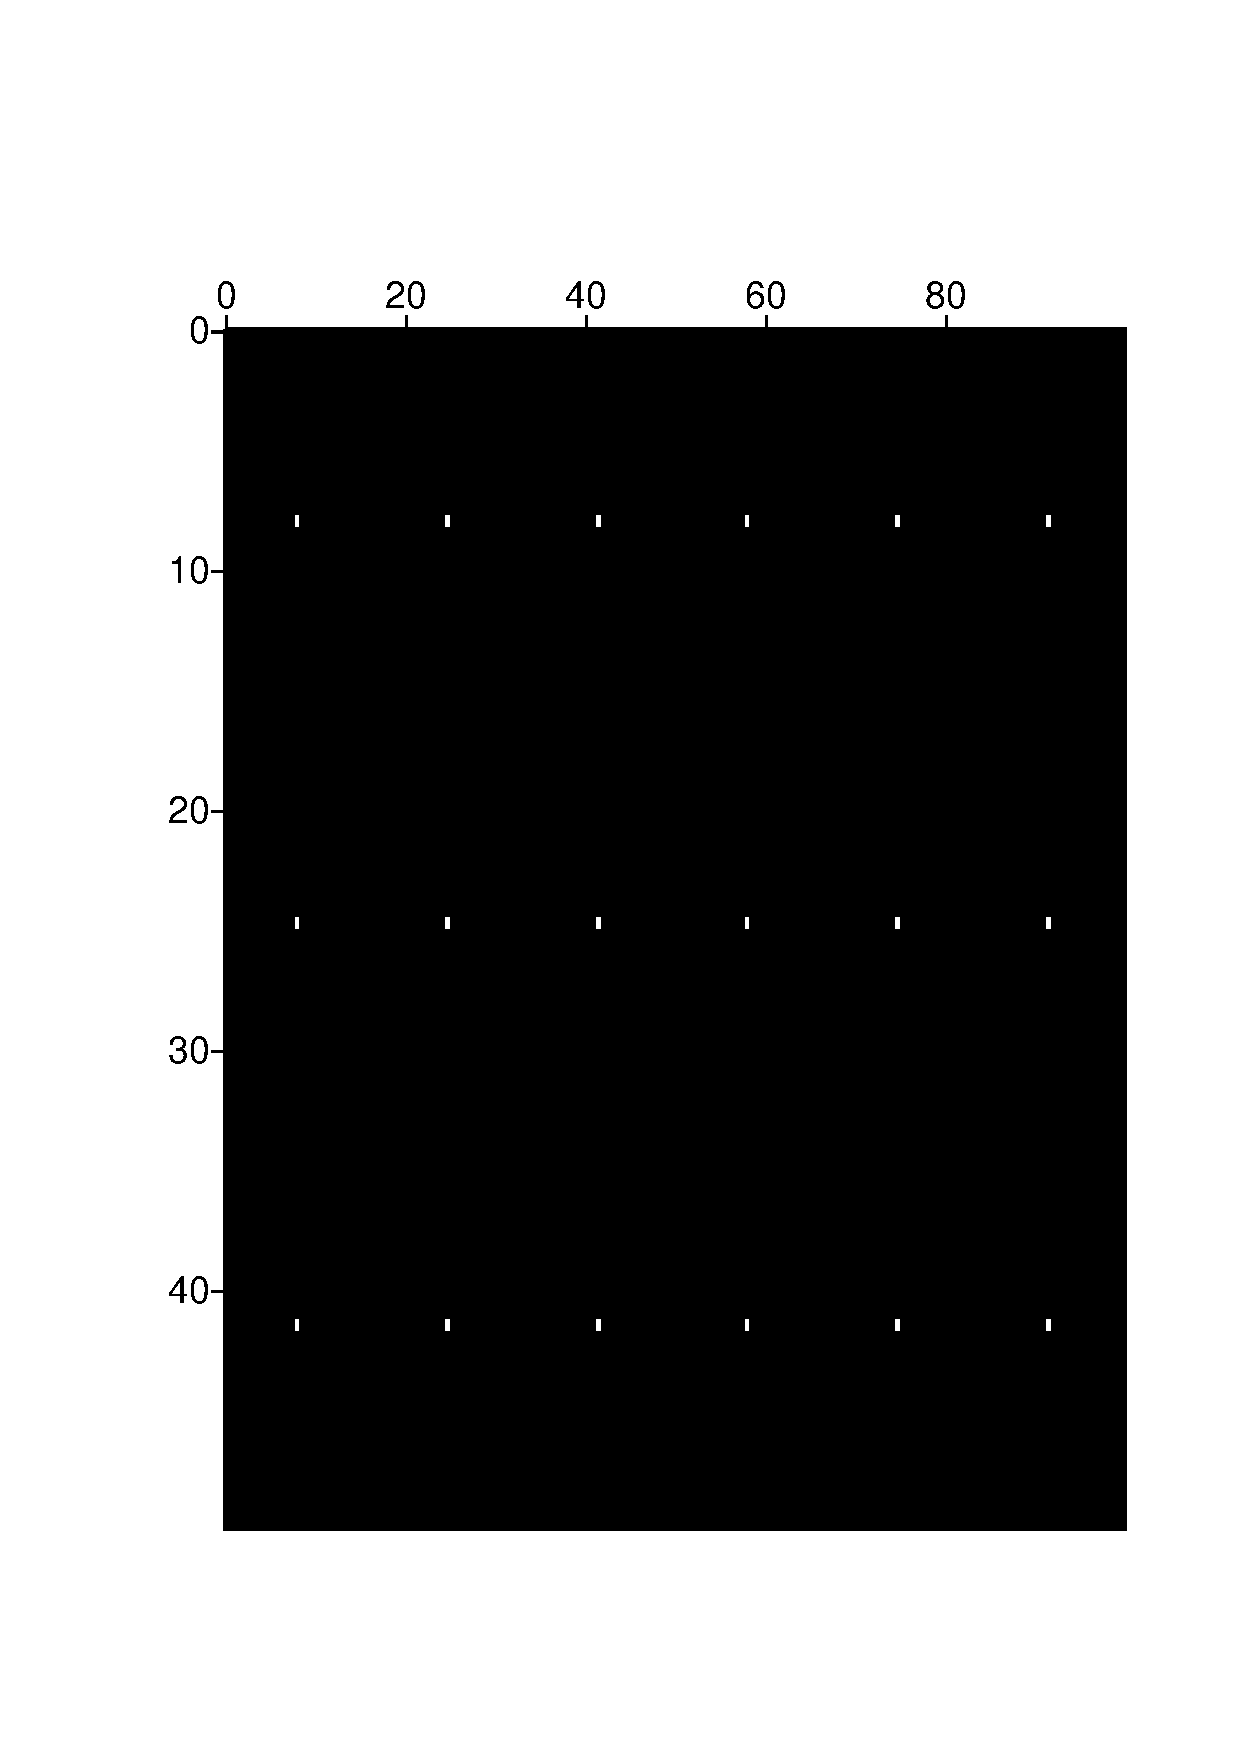
\includegraphics[height=5cm]{img/vp_scat.png}
	\caption{Configuration pour l'étude de résolution. La vitesse dans les inclusions est de 3000 m/s et de 6000 m/s ailleurs. Les éléments du transducteurs sont tous utilisés en réception et en transmission. \label{app:config_reso}}
\end{figure}


\subsection{Influence de la fréquence d'excitation}

Dans un premier temps, le milieu est entouré de conditions absorbantes. Les figures~\ref{app:150k} et~\ref{app:2M} montrent la couverture en nombres d'onde obtenue pour deux gammes de fréquence différentes. 
    
\begin{figure}[!h]
    \centering
    \begin{subfigure}[b]{0.05\textwidth}
 		\hspace{-2cm}\includegraphics[width=0.5cm]{img/echelle_fft.png}\vspace{2.1cm}
	\end{subfigure}
    \begin{subfigure}[b]{0.4\textwidth}
		\hspace{-3cm}\includegraphics[width=1.5\textwidth]{img/ssfreesurf_150k}
		\caption{Excitation centrée à 150 kHz.}
		\label{app:150k}
	\end{subfigure}	
	%\hspace{0.7cm}
	\begin{subfigure}[b]{0.4\textwidth}
		
\includegraphics[width=1.5\textwidth]{img/fft2d_nofreesurf_2MHz.png}
		\caption{Excitation centrée à 2 MHz.}
		\label{app:2M}
	\end{subfigure}
	\caption{Transformées de Fourier spatiales locales pour 2 gammes de fréquence d'excitation.}
\end{figure}

Comme l'indique l'expression de $k$ (équation~\ref{app:nb_onde}), pour une excitation basse fréquence, le gradient est pauvre en hauts nombres d'onde. Inversement, l'excitation haute fréquence ne permet pas de reconstruire les bas nombres d'onde.\\
La couverture en nombre d'onde est également très liée à l'acquisition. Elle est meilleure aux abords et en direction de la barrette. Les nombres d'onde verticaux seront globalement mieux reconstruits avec cette acquisition qui favorise les petits angles de diffraction, tandis que la couverture en nombres d'ondes horizontaux est très faible.

\subsection{Influence des surfaces libres}

Deux surfaces libres sont maintenant ajoutées à la soudure de référence et au modèle initial. L'objectif est d'illustrer l'influence de la durée du signal d'acquisition, soit le nombre de réflexions dans la plaques prises en compte dans les données. Les figures~\ref{app:1400pt} et~\ref{app:4200pt} montrent la couverture en nombres d'onde obtenue  pour 1 et 6 réflexions dans la plaque, pour une excitation à 2 MHz.

\begin{figure}[!h]
    \centering
    \begin{subfigure}[b]{0.05\textwidth}
 		\hspace{-2cm}\includegraphics[width=0.5cm]{img/echelle_fft.png}\vspace{2.1cm}
	\end{subfigure}
    \begin{subfigure}[b]{0.4\textwidth}
		\hspace{-3cm}\includegraphics[width=1.5\textwidth]{img/1400pt.png}
		\caption{Pour 1 réflexion, soit un trajet de 1 aller-retour dans l'épaisseur de la plaque.}
		\label{app:1400pt}
	\end{subfigure}	
	\hspace{0.7cm}
	\begin{subfigure}[b]{0.4\textwidth}
		\hspace{-0.7cm}\includegraphics[width=1.5\textwidth]{img/4200pt.png}
		\caption{Pour 6 réflexions, soit un trajet de 3 aller-retours dans l'épaisseur de la plaque.}
		\label{app:4200pt}
	\end{subfigure}
	\caption{Transformées de Fourier spatiales locales du gradient pour 2 durées d'acquisition. La fréquence d'excitation est centrée à 2 MHz.}
\end{figure}

Les surfaces libres sont assimilables à l'ajout de sources images éloignées qui favorisent une propagation verticale et de grands angles de diffraction (figure~\ref{app:reso_surf_libre}). Ainsi, les nombres d'onde horizontaux sont beaucoup mieux couverts avec, en contrepartie, une perte sur les nombres d'onde verticaux.  \\
Lorsque 6 réflexions sont prises en compte, l'ensemble des nombres d'ondes purement horizontaux est reconstruit, mais la résolution verticale est presque nulle.
\begin{figure}[!h]
	\centering
	\includegraphics[height=5cm]{img/reso_surf_libre.png}
	\caption{Illustration de l'impact d'une surface libre sur la résolution spatiale du gradient : la propagation verticale est favorisée, ainsi que les grands angles de diffraction.\label{app:reso_surf_libre}}
\end{figure}



Finalement, la prise en compte d'une réflexion dans les données d'acquisition permet d'améliorer la reconstruction des nombres d'onde horizontaux et donc la résolution latérale des défauts, tout en assurant une bonne couverture en nombres d'onde verticaux.


\section{Gestion des non-linéarités}
Une stratégie pour limiter la non-linéarité de l'inversion consiste à réaliser l'inversion en plusieurs temps, en injectant progressivement le contenu hautes fréquences dans les données. L'inversion à basses fréquences permet ainsi de reconstruire la structure grossière avant d'ajouter les détails grâce à la résolution qu'offre le gradient en hautes fréquences.\\



Afin que les nombres imagés soient correctement échantillonnés, il faut que le plus grand nombre d'onde imagé à une fréquence soit le même que le plus petit à la fréquence suivante \citep{sirgue}. En considérant que le plus bas nombre d'onde soit obtenu pour une angle de diffraction de 100° , le rapport de fréquences suivant doit donc être respecté : 

\begin{alignat*}{3}
	  ~&k_{max}(f_{n}) &&= k_{min}(f_{n+1})\\
	\Leftrightarrow~~~~~ &  f_n &&= f_{n+1}\cos \left(\frac{100^\circ}{2} \right)\\
	 \Leftrightarrow~~~~~ & \frac{f_{n+1}}{f_n} && \approx  1,5.
\end{alignat*} 

Les inversions présentées ci-après sont donc réalisées en plusieurs itérations. Entre chaque itérations, les données observées et l'ondelette d'excitation sont filtrées par un filtre passe-bas de fréquence centrale $f_{n}$ et dont la fréquence de coupure haute est de $2,5 \times f_{n}$.


\section{Inversions en milieu acoustique isotrope}

La méthode d'imagerie est appliquée à des milieux acoustiques, ce qui simplifie le problème et réduit les coûts de calcul. Le code utilisé est \emph{TOYxDacTIME}, développé dans le cadre du projet \emph{Seiscope}\footnote{http://seiscope2.osug.fr}. Le problème direct y est résolu par différences finies d'ordre 2 et l'inversion est réalisée dans le domaine temporel.\\
%, ce qui impose deux contraintes de discrétisation : dispersion numérique, cfl 

La propagation des ondes élastiques est décrite par les équations linéarisées en déplacements $\bm{u}$ et contraintes $\bar{\bar T}$ suivantes \citep{mat_ac2} : 

\begin{eqnarray}
	\rho \frac{\dd^2 u_{i}}{\dd t^2} &=& \displaystyle\sum_{j}\frac{\dd T_{ij}}{\dd x_{j}}\text{,}	\label{prop1}\\
	T_{ij}&=&\displaystyle\sum_{kl}C_{ijkl}\left( \frac{\dd u_{k}}{\dd x_{l}} + \frac{\dd u_{l}}{\dd x_{k}}\right)\text{,}	\label{prop2}
\end{eqnarray}
avec $C_{ijkl}$ le tenseur des constantes élastiques. Les études en milieu acoustique sont menées en approximation 2D : on suppose que le problème ne dépend pas de la dimension données par $\bm{e}_{y}$ (d'après l'orientation des axes indiquée en figure~\ref{BC}).\\

Les équations de la propagation acoustique peuvent être déduite de~\ref{prop1} et \ref{prop2} en considérant un module de cisaillement nul. On a alors $T_{ij}=0$ si $i\neq j$, ce qui donne le système :
\begin{eqnarray}
	\rho \frac{\dd^2 u_{i}}{\dd t^2} &=& \frac{\dd T_{ii}}{\dd x_{i}}\text{,}\\
	T_{ii} &=& \displaystyle\sum_{k}C_{iikk}\left( \frac{\dd u_{k}}{\dd x_{k}}\right)	.
\end{eqnarray}


On considère, tout d'abord, une propagation dans un milieu acoustique isotrope. Les constantes élastiques sont alors égales dans toutes les directions et les propriétés élastiques sont donc réduites à une seule constante. Les équations~\ref{prop1} et~\ref{prop2} deviennent : 
\begin{eqnarray}
	\rho \frac{\dd^2 u_{i}}{\dd t^2} = -\bm{\nabla} p \text{,}\\
	p=-\kappa \displaystyle\sum_{i} \frac{\dd u_{i}}{\dd x_{i}}\text{,}
\end{eqnarray}
avec $\kappa$ le module de rigidité et $p$ la pression.

Deux types d'inversions sont proposée par la suite pour une paramétrisation densité-vitesse du milieu : l'inversion monoparamètre, pour laquelle le modèle d'un seul des paramètres est mis à jour pendant que l'autre est maintenu constant, et l'inversion multiparamètre, pour laquelle les deux paramètres sont variables et mis à jour.


\subsection{Inversions monoparamètres}

 Dans un premier temps, on considère une configuration d'acquisition favorable à un bon éclairage de la soudure : deux barrettes linéaires de 64 éléments (en émission et réception) sont situées de part et d'autre de la soudure. Cette configuration ne correspond pas à celle d'une inspection de soudure conventionnelle, puisque en pratique, le relief de la soudure ne permet pas de placer les barrettes directement dessus. La durée d'acquisition est de 15,4 $\mu$s, ce qui correspond à une propagation sur 9 cm à 6000 m/s, soit moins d'un aller-retour dans l'épaisseur de la plaque. Les données observées sont calculées à partir du milieu dont la densité et  la vitesse verticale sont présentés en figure~\ref{app:iso:model}.\\


\begin{figure}[!h]
	\centering
	\begin{subfigure}[b]{0.45\textwidth}
		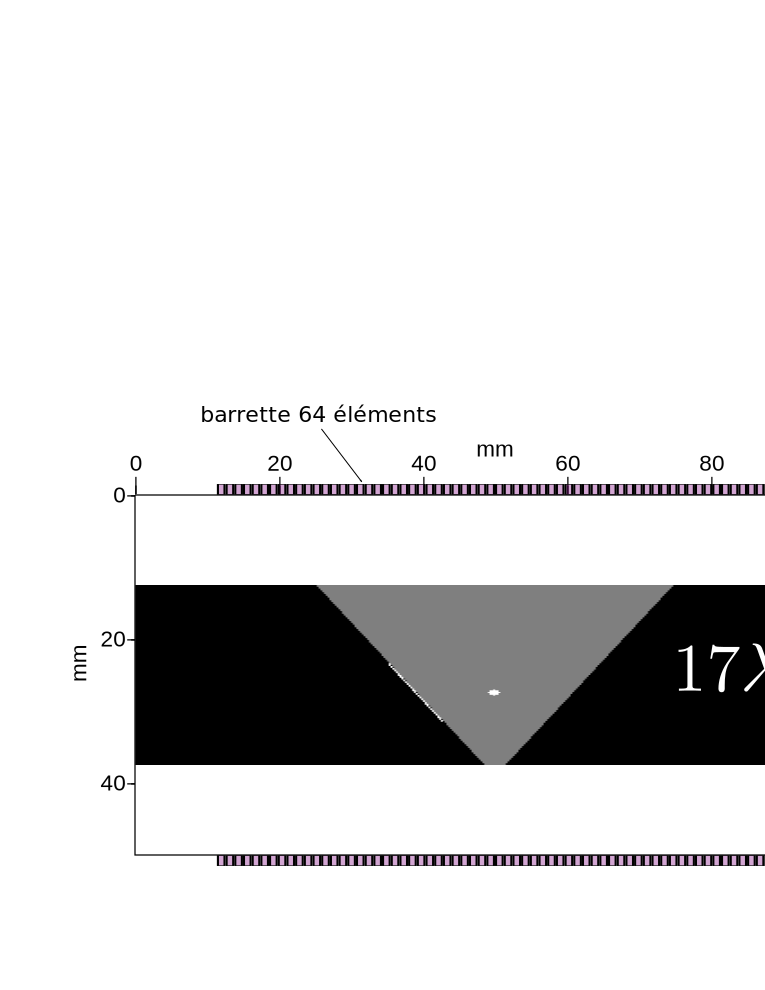
\includegraphics[width=\textwidth]{img/milieux_ps/vp_true.png}
		\caption{Vitesse vraie.}
	\end{subfigure}
	\begin{subfigure}[b]{0.45\textwidth}
		
\includegraphics[width=\textwidth]{img/milieux_ps/rho_true.png}
		\caption{Masse volumique vraie.}
	\end{subfigure}
	\caption{Milieux en vitesse et masse volumique pour la génération des données observées. Deux barrettes de 64 éléments sont utilisées en réception et en transmission, de part et d'autre de la soudure. La soudure simulée présente deux défauts : une inclusion de diamètre $\lambda/2$ et un manque de fusion de largeur $\lambda/12$.\label{app:iso:model}}
\end{figure}


Une première inversion est réalisée, en gardant $\rho$ à sa valeur initiale et en ne mettant à jour que le modèle de vitesse, pour 9 bandes de fréquences allant de 100 kHz à 3,4 MHz. Le modèle initial de vitesse pour cette inversion est pris uniforme avec $v_{p}=6000$~m/s.\\

Une seconde inversion monoparamètre est proposée pour une reconstruction de la masse volumique. Cependant, il est très difficile d'assurer une convergence en prenant des modèles initiaux de vitesse et de densité uniformes, car la seule mise à jour du modèle de densité ne peut expliquer la majeure partie des données en terme de cinématique. En effet, la figure~\ref{app:traces_rho} montre que la différence de densité au niveau des défauts n'impacte pas les temps de vol mais l'amplitude des diffractions sur les défauts. Il est donc nécessaire de disposer d'un modèle de vitesse suffisamment précis pour expliquer les différentes arrivées, puis la densité sera reconstruite par correction des amplitudes. Le modèle de vitesse initiale utilisé pour cette inversion est issue d'une première inversion de la vitesse avec un fort lissage gaussien de la perturbation sur deux longueurs d'onde.\\

Enfin, une autre inversion de la vitesse est réalisée, avec pour modèle initial ce même modèle de vitesse lissé et une densité uniforme, afin d'évaluer l'influence du modèle initial.\\

Les modèles initiaux de vitesse et le résultats de ces inversions se trouvent figure~\ref{app:inv_mono}. 


\begin{figure}
	\centering
	\begin{subfigure}[b]{0.45\textwidth}
		\centering
		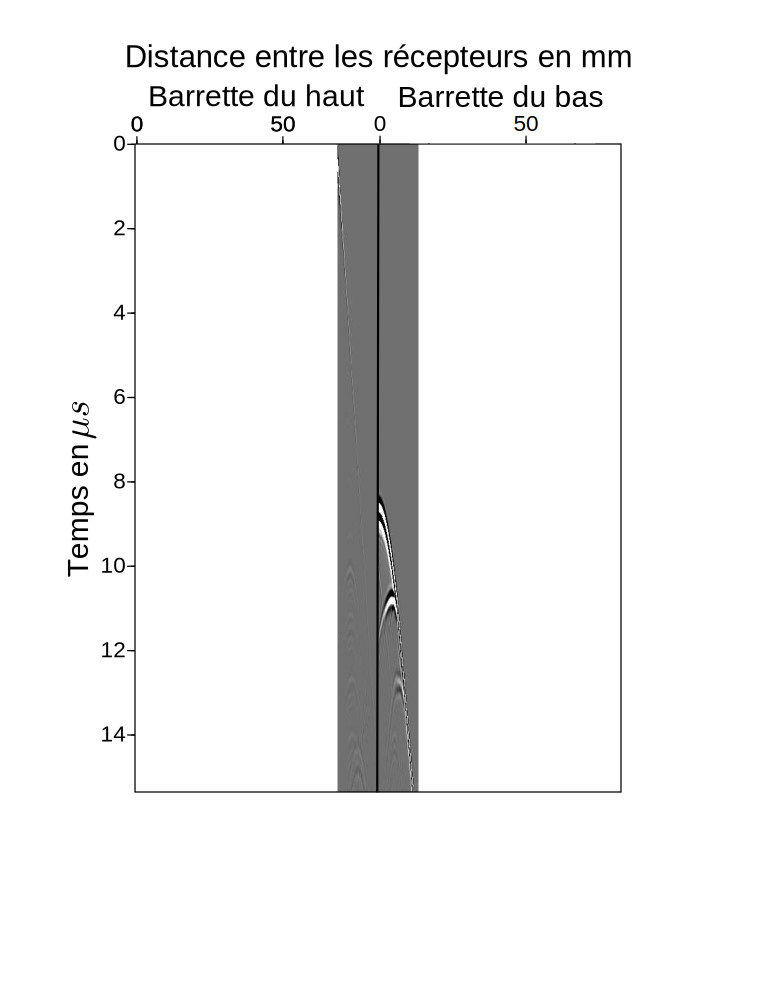
\includegraphics[width=0.8\textwidth]{img/rho_sur_donnees/data_rho_uni.png}
		\caption{Pour une densité uniforme.}
	\end{subfigure}
		\begin{subfigure}[b]{0.45\textwidth}
		\centering
		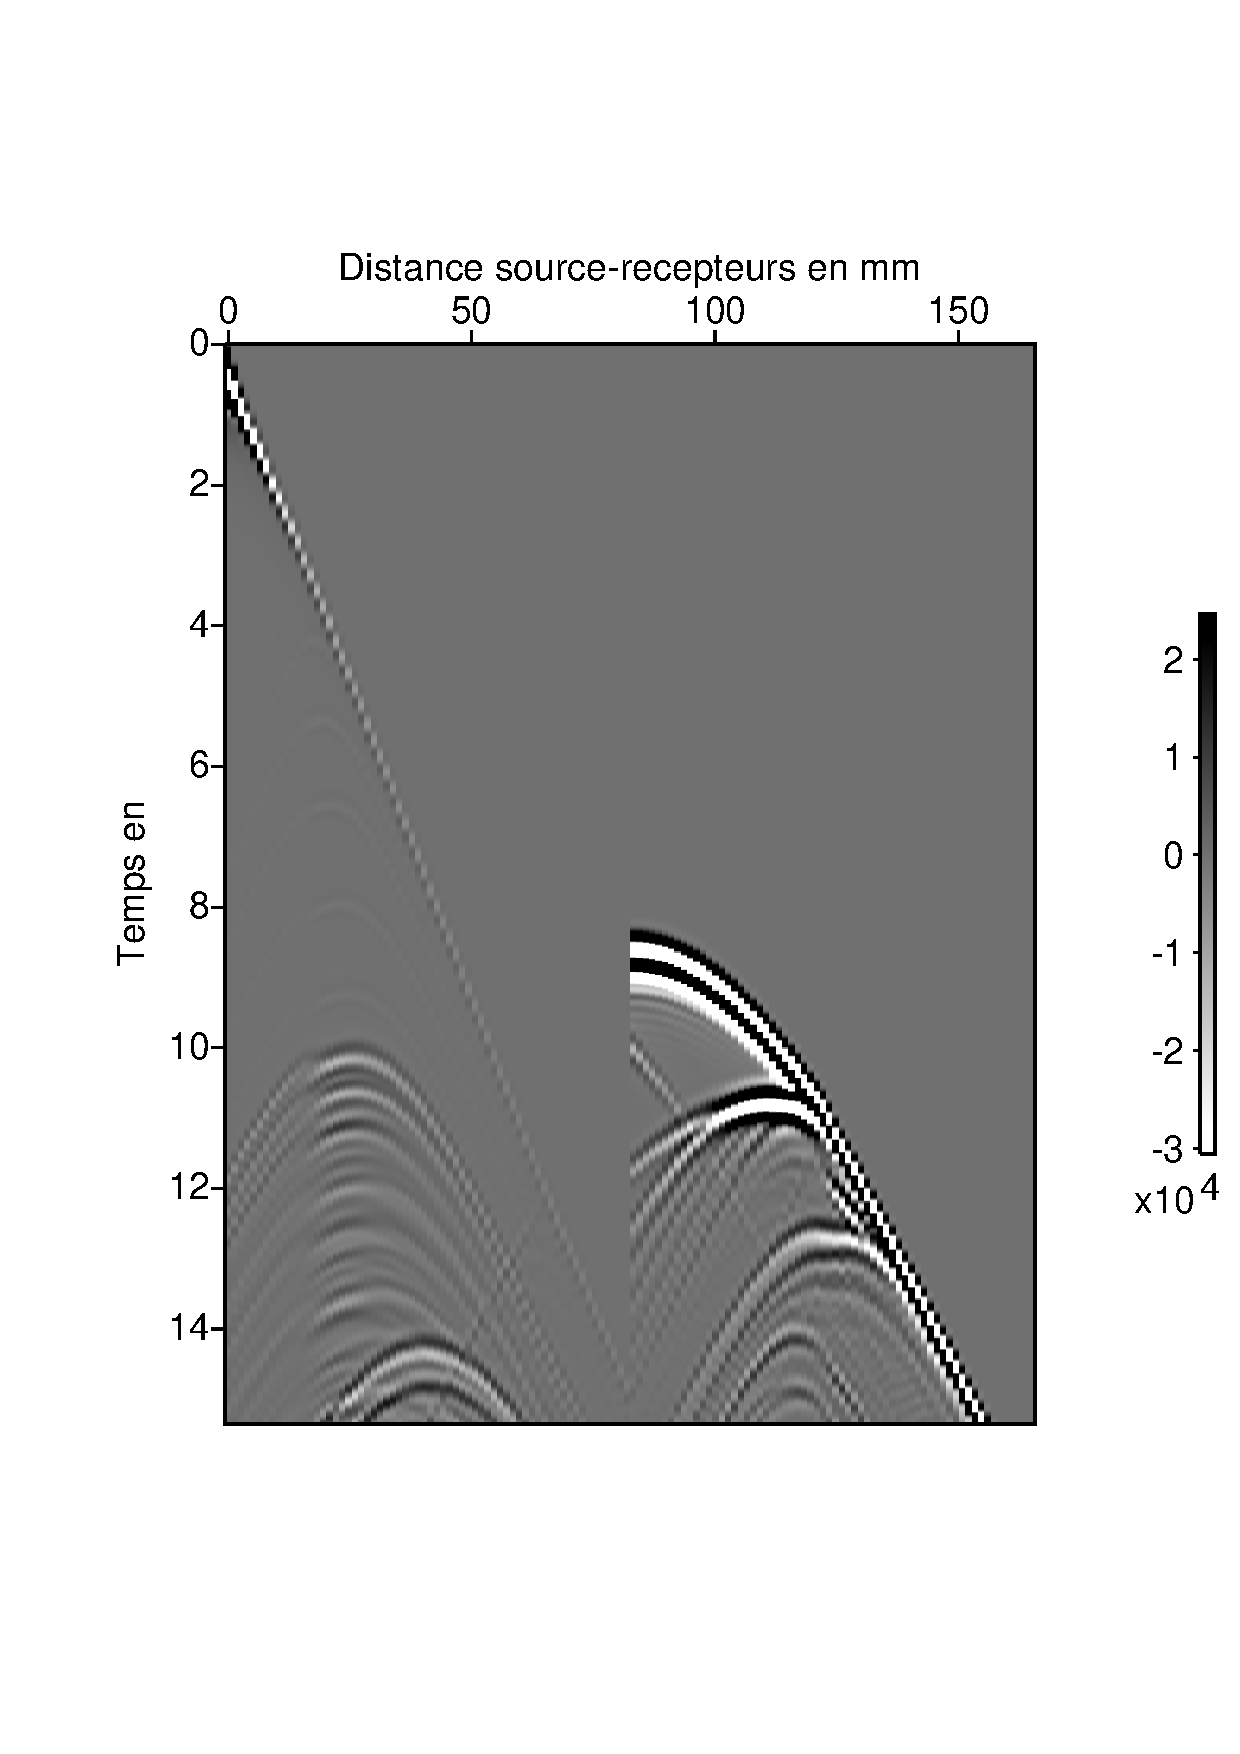
\includegraphics[width=0.8\textwidth]{img/rho_sur_donnees/data_rho_vrai.png}
		\caption{Pour $\rho=3000$~kg/m$^{3}$ dans les défauts.}
	\end{subfigure}
	\caption{Effet du contraste de densité sur les données observées (même échelle d'amplitude) : les temps de vol ne sont pas impactés, mais l'amplitude de l'onde diffractée est plus importante en présence du contraste de densité. \label{app:traces_rho}}	
\end{figure}



	\begin{figure}[p]
	\begin{changemargin}{-2cm}{-2cm}
		\centering
		\begin{subfigure}[b]{0.29\textwidth}
			\centering
			Première inversion de la vitesse : \\[0.2cm]
			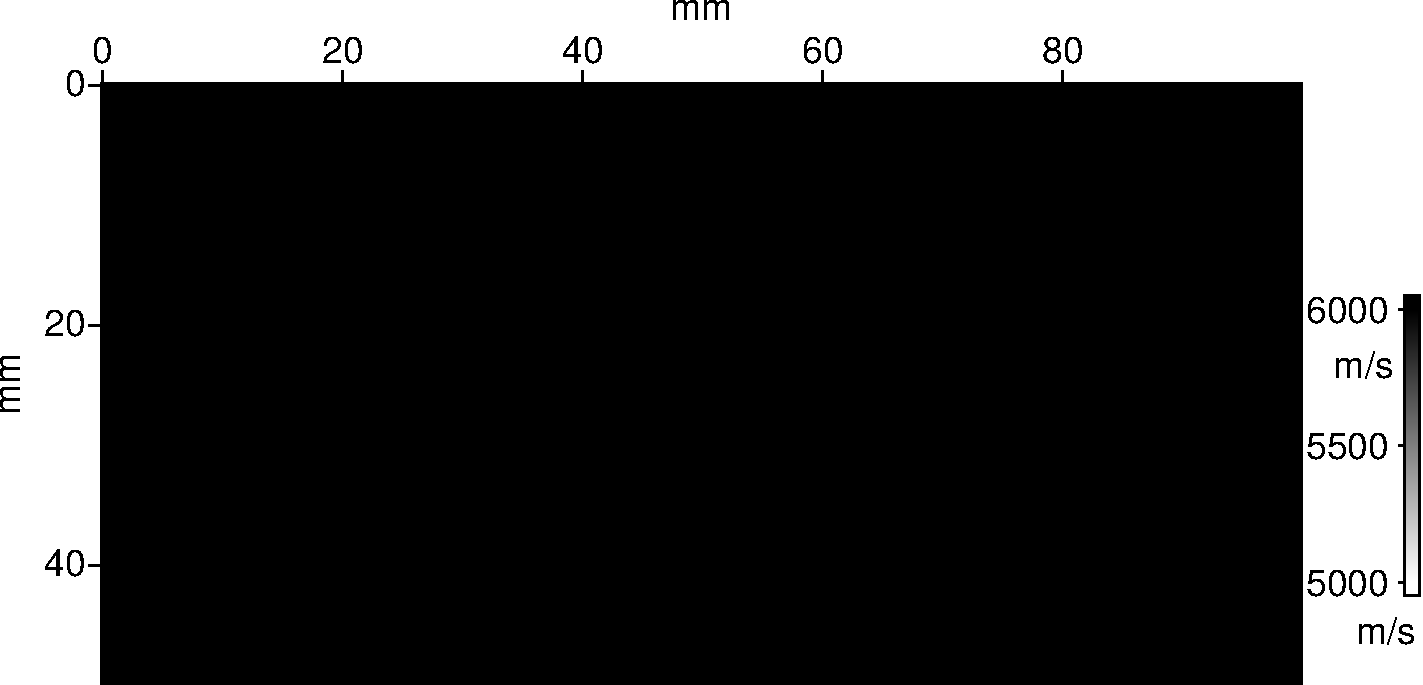
\includegraphics[width=\textwidth]{img/mono_param/vp_uni.png}
			\caption{Modèle de vitesse initial.}
		\end{subfigure}
		\begin{subfigure}[b]{0.29\textwidth}
			\centering
			Seconde inversion de la vitesse : \\[0.2cm] 
			\includegraphics[width=\textwidth]{img/mono_param/vp_smooth.png}
			\caption{Modèle de vitesse initial.}
		\end{subfigure}
		\begin{subfigure}[b]{0.29\textwidth}
			\centering
			Inversion de la masse volumique :  \\[0.2cm]
			\includegraphics[width=\textwidth]{img/mono_param/vp_smooth.png}
			\caption{Modèle de vitesse initial.}
		\end{subfigure}
		\begin{subfigure}[b]{0.29\textwidth}
			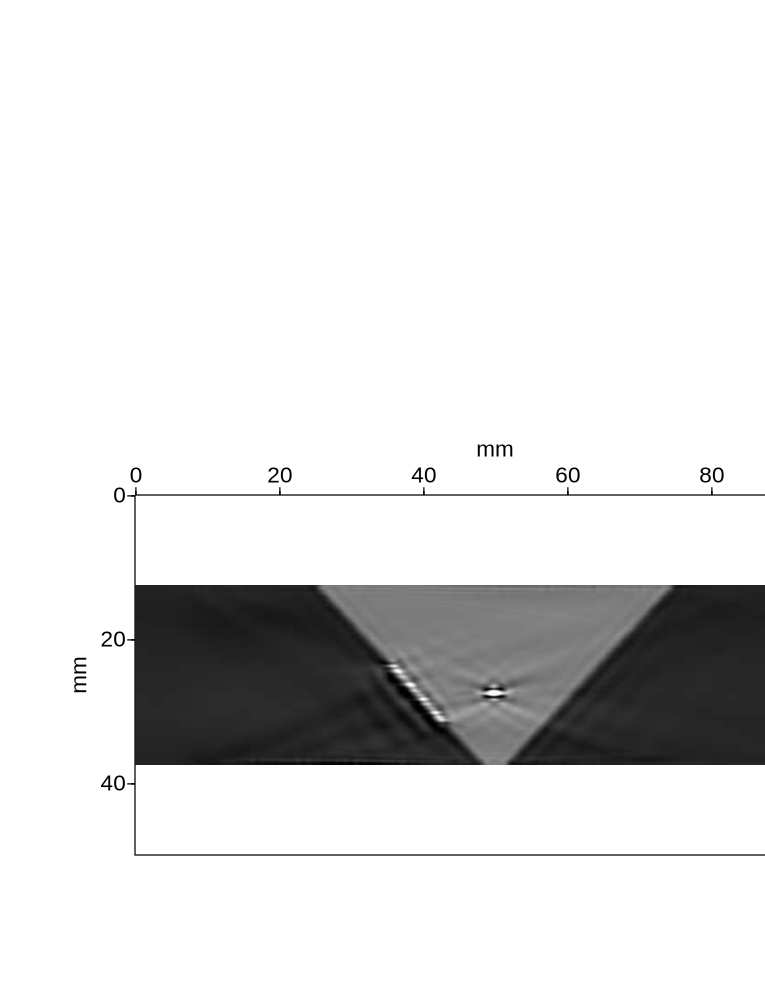
\includegraphics[width=\textwidth]{img/mono_param/vp_final_uni.png}
			\caption{Vitesse reconstruite par FWI monoparamètre.}
		\end{subfigure}
		\begin{subfigure}[b]{0.29\textwidth}
			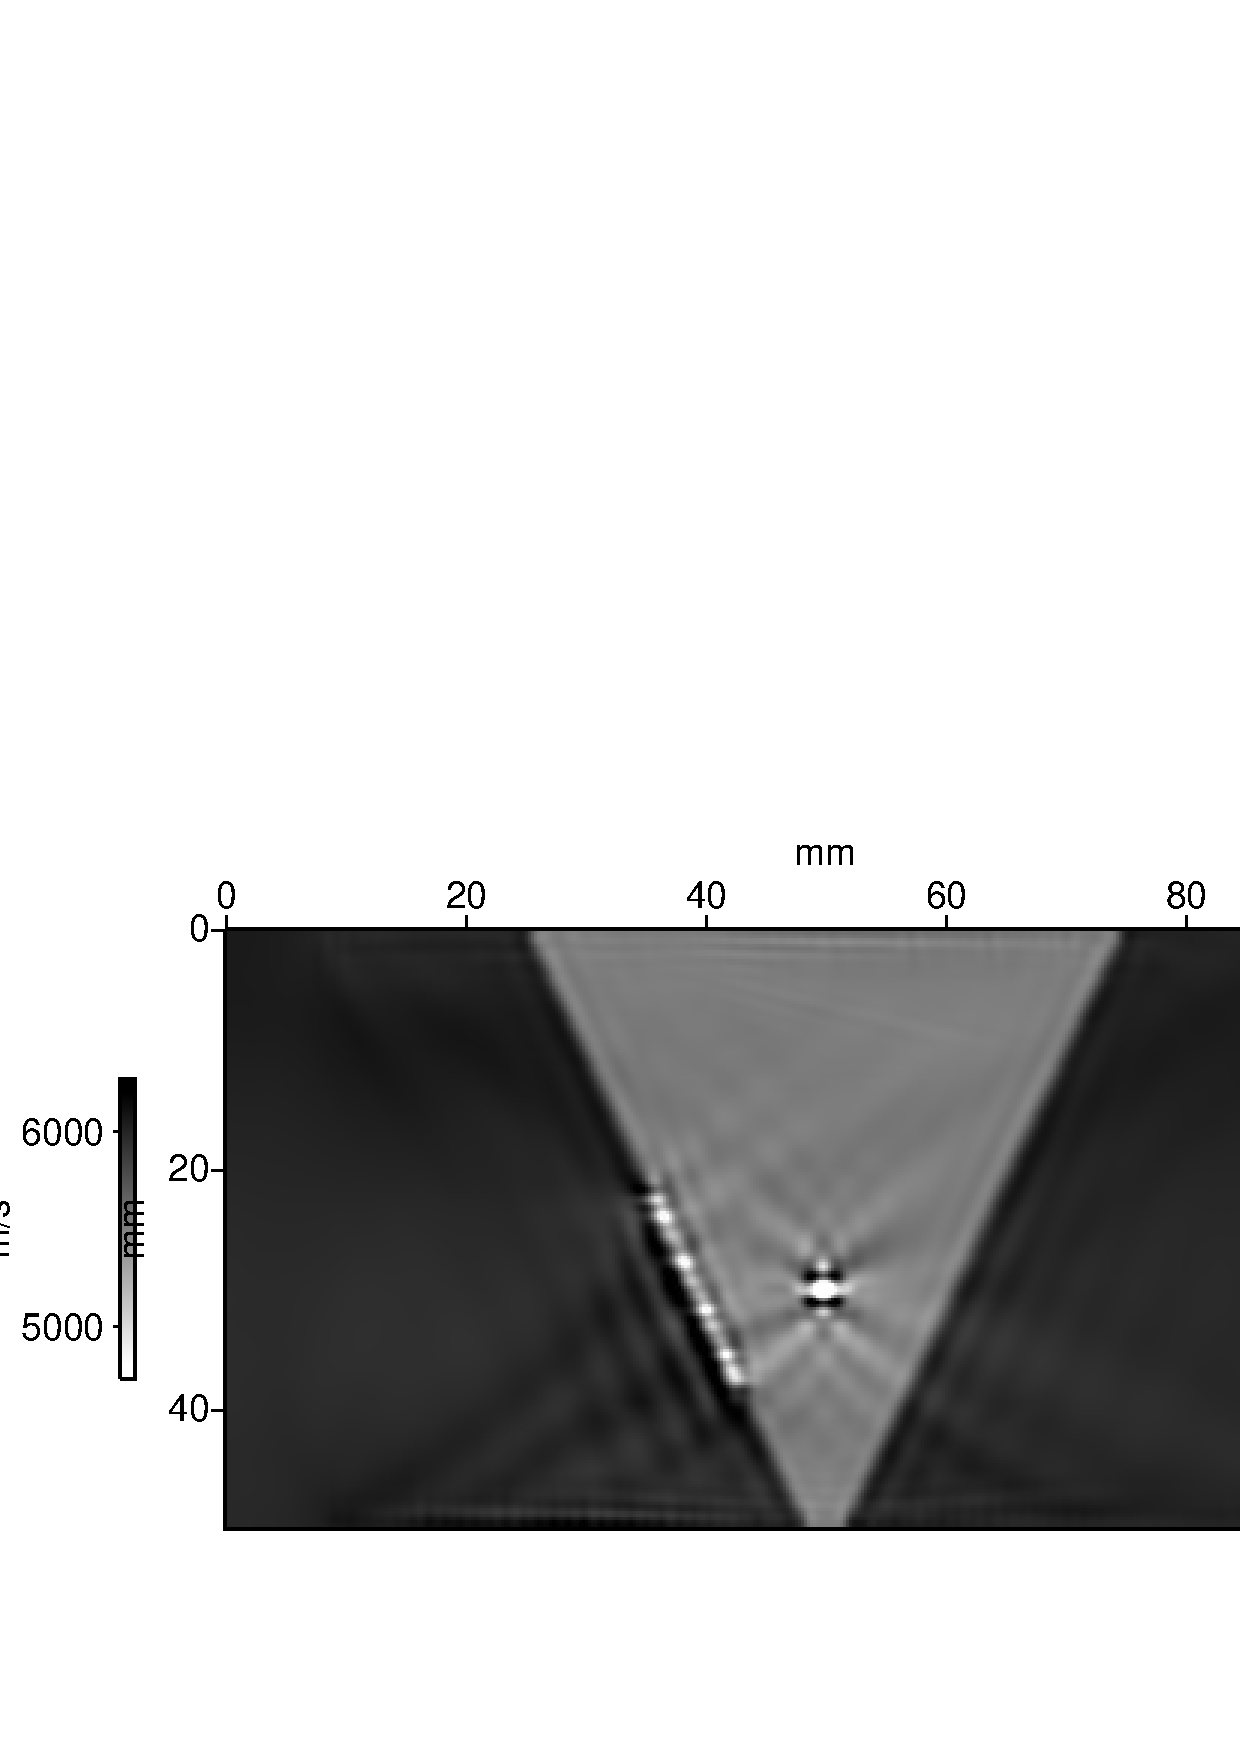
\includegraphics[width=\textwidth]{img/mono_param/vp_final_smooth.png}
			\caption{Vitesse reconstruite par FWI monoparamètre.}
		\end{subfigure}
		\begin{subfigure}[b]{0.29\textwidth}
			
\includegraphics[width=\textwidth]{img/mono_param/rho_mono.png}
			\caption{Masse volumique reconstruite par FWI monoparamètre.}
		\end{subfigure}
		\begin{subfigure}[b]{0.29\textwidth}
			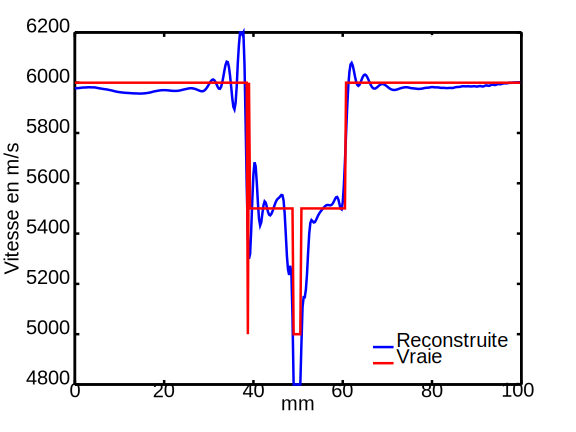
\includegraphics[width=\textwidth]{img/mono_param/coupe_vp_mono_uni_hor.png}
			\caption{Vitesses vraie et vitesse reconstruite à $y=30$~mm.}
		\end{subfigure}
		\begin{subfigure}[b]{0.29\textwidth}
			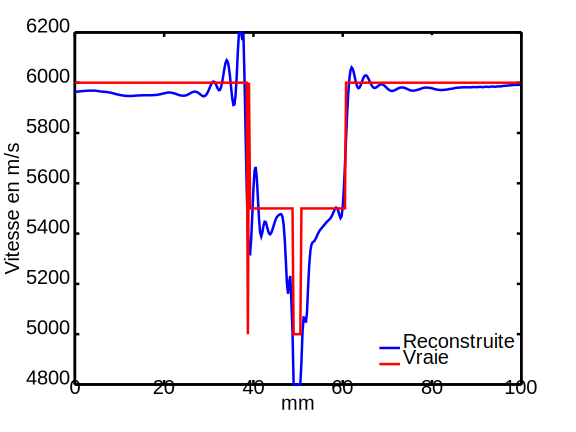
\includegraphics[width=\textwidth]{img/mono_param/coupe_vp_mono_smooth_hor.png}
			\caption{Vitesses vraie et vitesse reconstruite à $y=30$~mm.}
		\end{subfigure}
		\begin{subfigure}[b]{0.29\textwidth}
			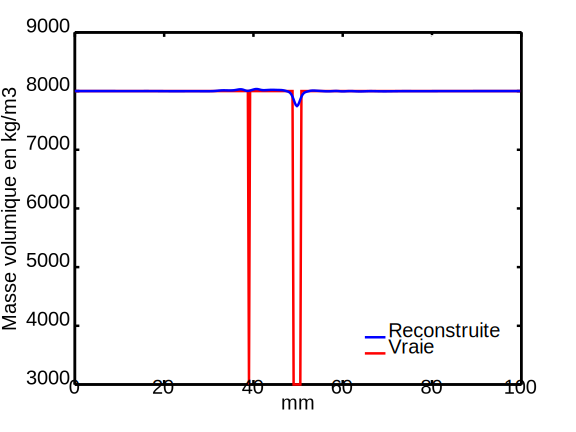
\includegraphics[width=\textwidth]{img/mono_param/coupe_rho_mono.png}
			\caption{Masses volumiques vraie et reconstruite à $y=30$~mm.}
		\end{subfigure}
				\begin{subfigure}[b]{0.29\textwidth}
			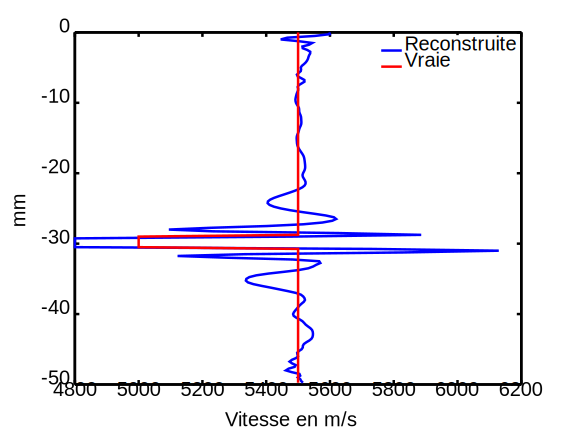
\includegraphics[width=\textwidth]{img/mono_param/coupe_vp_mono_uni_vert.png}
			\caption{Vitesses vraie et vitesse reconstruite à $x=50$~mm.}
		\end{subfigure}
		\begin{subfigure}[b]{0.29\textwidth}
			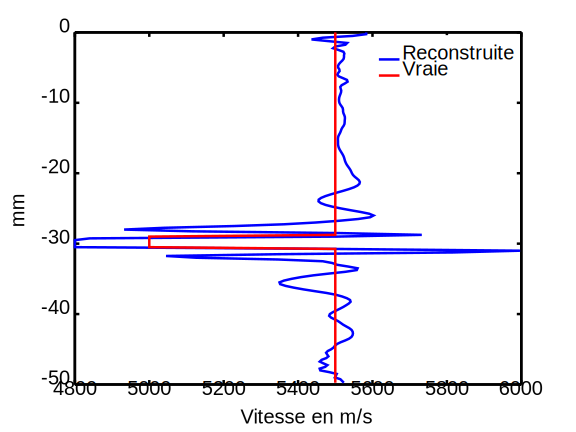
\includegraphics[width=\textwidth]{img/mono_param/coupe_vp_mono_smooth_vert.png}
			\caption{Vitesses vraie et vitesse reconstruite à $x=50$~mm.}
		\end{subfigure}
		\begin{subfigure}[b]{0.29\textwidth}
			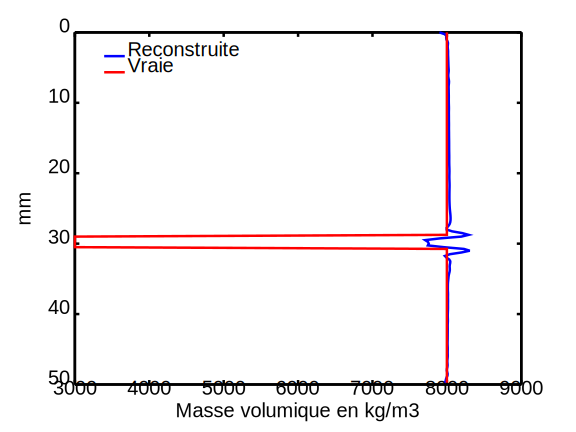
\includegraphics[width=\textwidth]{img/mono_param/coupe_rho_mono_vert.png}
			\caption{Masses volumiques vraie et reconstruite à $x=50$~mm.}
		\end{subfigure}
		\caption{\label{app:inv_mono} Modèle initiaux de vitesse et résultat d'inversion monoparamètre de la vitesse (deux colonnes de gauche) et de la densité (colonne de droite).}
	\end{changemargin}
	\end{figure}

Pour l'inversion de la vitesse, le modèle initial plus précis permet d'obtenir des résultats d'inversion plus précis et plus rapidement, à basses fréquences seulement. À partir de 1.5 MHz, les modèles courants de vitesse deviennent semblables. C'est à cette fréquence qu'apparaissent progressivement  des artefacts hautes fréquences, malgré un lissage gaussien de 0.8 longueur d'onde. Dans ces conditions, le résultat final n'est donc pas influencé par le choix du modèle initial. La section verticale des vitesses reconstruites manque de bas nombres d'ondes en raison de la largeur limitée des barrettes.\\


Les bords latéraux des défauts reconstruits par la masse volumique ne sont pas précisément définis. L'acquisition devrait favoriser une reconstruction des nombres d'ondes horizontaux, mais le diagramme de rayonnement de la densité pour la paramétrisation $v_{p}-\rho$ montre que la densité n'est pas prompt à décrire le rayonnement latéral de la diffraction. La coupe horizontale à 3 cm de profondeur présente donc un manque de hauts nombres d'onde. De manière générale, ce paramètre est moins bien reconstruit que la vitesse en amplitude, en raison de son faible impact sur les données observées. Une image précise de la densité pourrait permettre de caractériser plus précisément certains types de défauts, et il faudrait alors pondérer ce paramètre de façon à donner plus de poids à sa perturbation.\\


\subsubsection{Exemple d'acquisition réaliste}
Un exemple d'inversion monoparamètre de la vitesse est présenté ici, à partir d'une acquisition plus réaliste. Deux barrettes de 64 éléments espacés de 1 mm sont placées de chaque côté de la racine de la soudure. Les données sont générée à partir d'une soudure de densité uniforme et de vitesse présentée en figure~\ref{app:iso:reel1}. La durée des signaux acquis est de 30.7 $\mu s$, ce qui est le temps nécessaire à la propagation d'une extrémité à l'autre du système d'acquisition. Le modèle initial de vitesse est uniforme, avec $v_{p}=6000$~m/s.\\

 Le résultat de l'inversion, réalisée sur des fréquences de 200 k à 5 MHz et présenté en figure~\ref{app:iso:reel2}, illustre à nouveau la dépendance de la résolution vis à vis du système d'acquisition. En effet, la racine de la soudure est mal reconstruite dans cette zone car les diffractions mesurées sont d'angle nul ou proche de $\pi$. Or, les angles de diffraction proches de $\pi$  contribuent à une reconstruction de résolution très faible, d'après l'expression du nombre d'onde~\ref{app:nb_onde}. Pour une application de la FWI à un cas réel, il est donc nécessaire de déterminer au préalable l'acquisition favorisant un éclairage adapté à la géométrie de la pièce à évaluer.
 
\begin{figure}
	\begin{subfigure}[b]{0.5\textwidth}
		\centering
		\includegraphics[width=\textwidth]{img/config_reelle_true.png}
		\caption{Configuration du système d'acquisition et vitesse utilisée pour la génération des données.\label{app:iso:reel1}}	
	\end{subfigure}
	\hspace{0.2cm}
	\begin{subfigure}[b]{0.5\textwidth}
		\centering
		\includegraphics[width=\textwidth]{img/config_reelle_rec.png}
		\caption{Vitesse reconstruite par inversion monoparamètre. \label{app:iso:reel2}}	
	\end{subfigure}
	\caption{Exemple d'inversion pour une acquisition unilatérale. Chaque barrette est utilisée en excitation et en réception.}
\end{figure}

\subsection{Inversion multiparamètre}

Lors d'une inversion multiparamètre, les modèles des différents paramètres sont mis à jour simultanément. Idéalement, cela permet de perturber chaque modèle de façon à expliquer au mieux l'effet de chaque paramètre sur les données. Cependant, il arrive que ces effets soient attribué à de mauvais paramètres dont le modèle est alors faussement perturbé. Dans le cas d'une paramétrisation $v_{p}-\rho$, le risque est que la densité soit perturbée de façon à expliquer des temps de vol, ce qui ne permettra jamais de tendre vers le milieu vrai. Il est donc préférable, dans un premier temps, d'inverser seul le paramètre d'effet dominant dans les données, puis d'inverser conjointement l'ensemble des paramètres.\\

 Dans notre cas, le paramètre dominant est $v_{p}$, comme le montre la figure~\ref{app:traces_rho}. La stratégie est donc d'inverser ce paramètre à basse fréquence et avec un fort lissage, afin d'obtenir d'un modèle qui explique la majorité des arrivées. La vitesse et la densité sont ensuite reconstruites par FWI à partir de ce modèle de vitesse grossier. \\
 
Les données utilisées sont celles issues du modèle et de l'acquisition de la figure~\ref{app:iso:model}.  Le résultat de cette inversion multiparamètre est présenté en figure~\ref{app:inv_multi}. 
\\

L'inversion multiparamètre semble moins sujette aux artefacts (à lissage équivalent) \todo{Pourquoi ?} et permet une reconstruction des bords des défauts plus fine. L'inversion multiparamètre donne également plus de poids au paramètre de densité dont l'amplitude est légèrement mieux reconstruite qu'en inversion monoparamètre.  




\begin{figure}[!h]
	\centering
	\begin{subfigure}[b]{0.40\textwidth}
		\includegraphics[width=\textwidth]{img/multi_param/vp_smooth.png}
		\caption{Modèle initial de vitesse.}
	\end{subfigure}\\
%	\begin{subfigure}[b]{0.45\textwidth}
%		
\includegraphics[width=\textwidth]{img/multi_param/rho_init.png}
%		\caption{}
%	\end{subfigure}
	\begin{subfigure}[b]{0.4\textwidth}
		\includegraphics[width=\textwidth]{img/multi_param/vp_multi_6000k.png}
		\caption{Modèle final de vitesse obtenu par FWI multiparamètre.}
	\end{subfigure}
	\begin{subfigure}[b]{0.4\textwidth}
		
\includegraphics[width=\textwidth]{img/multi_param/rho_6000k.png}
		\caption{Modèle final de densité obtenu par FWI multiparamètre.}
	\end{subfigure}
	\begin{subfigure}[b]{0.4\textwidth}
		\includegraphics[width=\textwidth]{img/multi_param/coupe_vp_multi.png}
		\caption{Vitesses vraie et vitesse reconstruite à $y=30$~mm.}
	\end{subfigure}
	\begin{subfigure}[b]{0.4\textwidth}
		\includegraphics[width=\textwidth]{img/multi_param/coupe_rho_multi.png}
		\caption{Masse volumiques vraie et reconstruite à $y=30$~mm.}
	\end{subfigure}
	\begin{subfigure}[b]{0.4\textwidth}
		\includegraphics[width=\textwidth]{img/multi_param/coupe_vp_multi_vert.png}
		\caption{Vitesses vraie et reconstruite à $x=50$~mm.}
	\end{subfigure}
	\begin{subfigure}[b]{0.4\textwidth}
		\includegraphics[width=\textwidth]{img/multi_param/coupe_rho_multi_vert.png}
		\caption{Masses volumiques vraie et reconstruite à $x=50$~mm.}
	\end{subfigure}
	\caption{Modèle initial de vitesse et résultats d'inversion multiparamètre de la vitesse et de la densité.\label{app:inv_multi} }
\end{figure}






\section{Inversions en milieu acoustique transverse isotrope}
Afin d'introduire une anisotropie simplifiée dans la soudure, une étude dans un milieu acoustique vertical transverse isotrope est menée.
Il est possible de formuler à partir des équations de la propagation élastique~\ref{prop1} et~\ref{prop2} des équations d'ondes acoustiques en milieu anisotrope. Bien que ce soit physiquement impossible, cette formulation permet de se rapprocher cinématiquement des équations d'ondes élastiques, de manière simplifiée \citep{alkhalifah}.\\
En milieu transverse isotrope, la matrice des constantes élastiques est telles que  : 

\begin{equation}
	C_{iikk} = \begin{pmatrix}
		c_{11} & c_{12} & c_{13} & 0 & 0 & 0 \\
		c_{12} & c_{11} & c_{13} & 0 & 0 & 0 \\
		c_{13} & c_{13} & c_{33} & 0 & 0 & 0 \\
		0 & 0 & 0 & c_{44} & 0 & 0 \\
		0 & 0 & 0 & 0 &c_{44} & 0 \\
		0 & 0 & 0 & 0 & 0 & c_{66} = \frac{c_{11}-c_{12}}{2}
	\end{pmatrix}.
\end{equation}
L'approximation acoustique des équations élastiques en milieu vertical transverse isotrope (VTI) impose que $c_{66}$=0, soit $c_{11}=c_{12}$.
 

La paramétrisation du milieu peut donc se faire à l'aide de 4 constantes, que l'on choisit comme étant la vitesse verticale des ondes de compression $v_{p}$, la masse volumique $\rho$ et deux constantes adimensionnelles de Thomsen~\citep{thomsen} (surtout utilisées dans le domaine des Sciences de la Terre) définies comme suit : 
\begin{eqnarray}
	\epsilon & =  & \frac{C_{11}-C_{33}}{2C_{33}} = \frac{\bm{v}_{p}.\bm{e}_{x} -  \bm{v}_{p}.\bm{e}_{z}}{\bm{v}_{p}.\bm{e}_{z}},\\
	\delta & = & \frac{(C_{13}+C_{44})^2-(C_{33}-C_{44})^2}{2C_{33}(C_{33-C_{44}})}\text{.}
\end{eqnarray}

Le paramètre $\epsilon$ est donc lié à la différence entre la composante verticale et la composante horizontale de la vitesse des ondes de compression et $\delta$ décrit davantage la propagation des ondes quasi-longitudinales.\\

Notons que cette formulation peut notamment générer, en milieu anelliptique, un artefact d'onde de cisaillement, nettement visible sur les données synthétiques en figure~\ref{app:ani:data_true}. Il existe plusieurs stratégie pour limiter ces artefacts \citep{duveneck}, et il est choisi par la suite de simplement l'enlever des données par un filtre spatio-temporel.\\


%Notons que cette formulation [Pose quelques problèmes (Duveneck 2008) notamment génération d'onde S (sur données "vrai simulée"  et sur problème direct, mais pas la même car différente grille, PML, ... donc on la mute sur le résidu) qui n'a pas de sens physique. Proposer les solutions (taper Epsilon, en sismo on est dans l'eau donc c'est fait naturellement -> placer les sources dans un milieu isotrope).]




Pour la génération des données synthétiques, on considère une plaque isotrope dans laquelle se trouve une soudure anisotrope VTI sans défaut. La valeur de $\epsilon$ dans la soudure est fixée à 20~\%, ce qui est environ deux fois plus élevé que les valeurs que l'on peut trouver dans la littérature~\citep{chassignole}. 
Les barrettes, utilisées en réception et en transmission  sont placées de manière éloignée, afin d'accentuer la propagation des ondes suivant $\bm{e}_{x}$ et de s'assurer que les temps de vol soient perturbés par l'anisotropie (figure~\ref{configuration_vti}). Elles sont constituées de 16 éléments espacés de 1 mm.\\
Les autres paramètres ($v_{p}$, $\rho$ et $\delta$) sont choisis uniformes pour la génération des données et sont maintenus à leur valeur vraie pendant l'inversion, avec $v_{p}=6000$~m/s, $\rho=8000$~kg/m$^3$ et $\delta=0$.\\


L'inversion est réalisée à partir d'un modèle initial pour $\epsilon$ uniformément nul. Dès les premières inversions à 100 kHz, le modèle courant est grossièrement modifié, ce qui corrige légèrement les retards dus à l'anisotropie. Les itérations suivantes ne modifient presque pas le modèle courant, ce qui implique que la vallée de la fonction est coût très large. Le résultat de l'inversion à 500 kHz est présenté en figure~\ref{app:ani:res} et les résidus, avant et après inversion, sont confrontés en figures~\ref{app:ani:data_av} et~\ref{app:ani:data_ap}. \\


Les résidus issus du modèle initial ($\epsilon$ uniformément nul) montrent que ce paramètre change principalement la vitesse des ondes directes et réfléchies et cause peu de diffraction sur les bords de la soudure. Les trajets les plus impactés par l'anisotropie VTI, et donc les plus susceptibles de contribuer à la reconstruction du paramètre $\epsilon$, sont les trajets horizontaux, très difficiles à favoriser en excitation de surface. L'acquisition permet alors de mesurer les diffractions d'angles $\theta$ très faibles ou proches de $\pi$. Or, la résolution est très mauvaise pour $\theta=\pi$, d'après l'expression du nombre d'onde~\ref{app:nb_onde}.  

\begin{figure}[!h]
	\begin{subfigure}[b]{0.5\textwidth}
		\centering
		
\includegraphics[width=\textwidth]{img/epsilon/epsilon_true.png}
		\caption{Valeur du paramètre $\epsilon$ pour la génération des données observées. \label{configuration_vti} }
	\end{subfigure}
	\begin{subfigure}[b]{0.5\textwidth}
		\centering
		
\includegraphics[width=\textwidth]{img/epsilon/epsilon_final.png}\\
		\vspace{0.4cm}
		\caption{Résultat d'inversion monoparamètre du paramètre $\epsilon$.\label{app:ani:res}}
	\end{subfigure}	
	\caption{Milieu vrai et milieu reconstruit par FWI. L'inversion est réalisée à partir d'une valeur de $\epsilon$ uniformément nulle, de 100 à 500 kHz.}
\end{figure}

\begin{figure}[h!]
	\begin{changemargin}{-1cm}{-2cm}
	%donnees vraies, residus initiaux, residus finaux
	\begin{subfigure}[b]{0.29\textwidth}
		\centering
		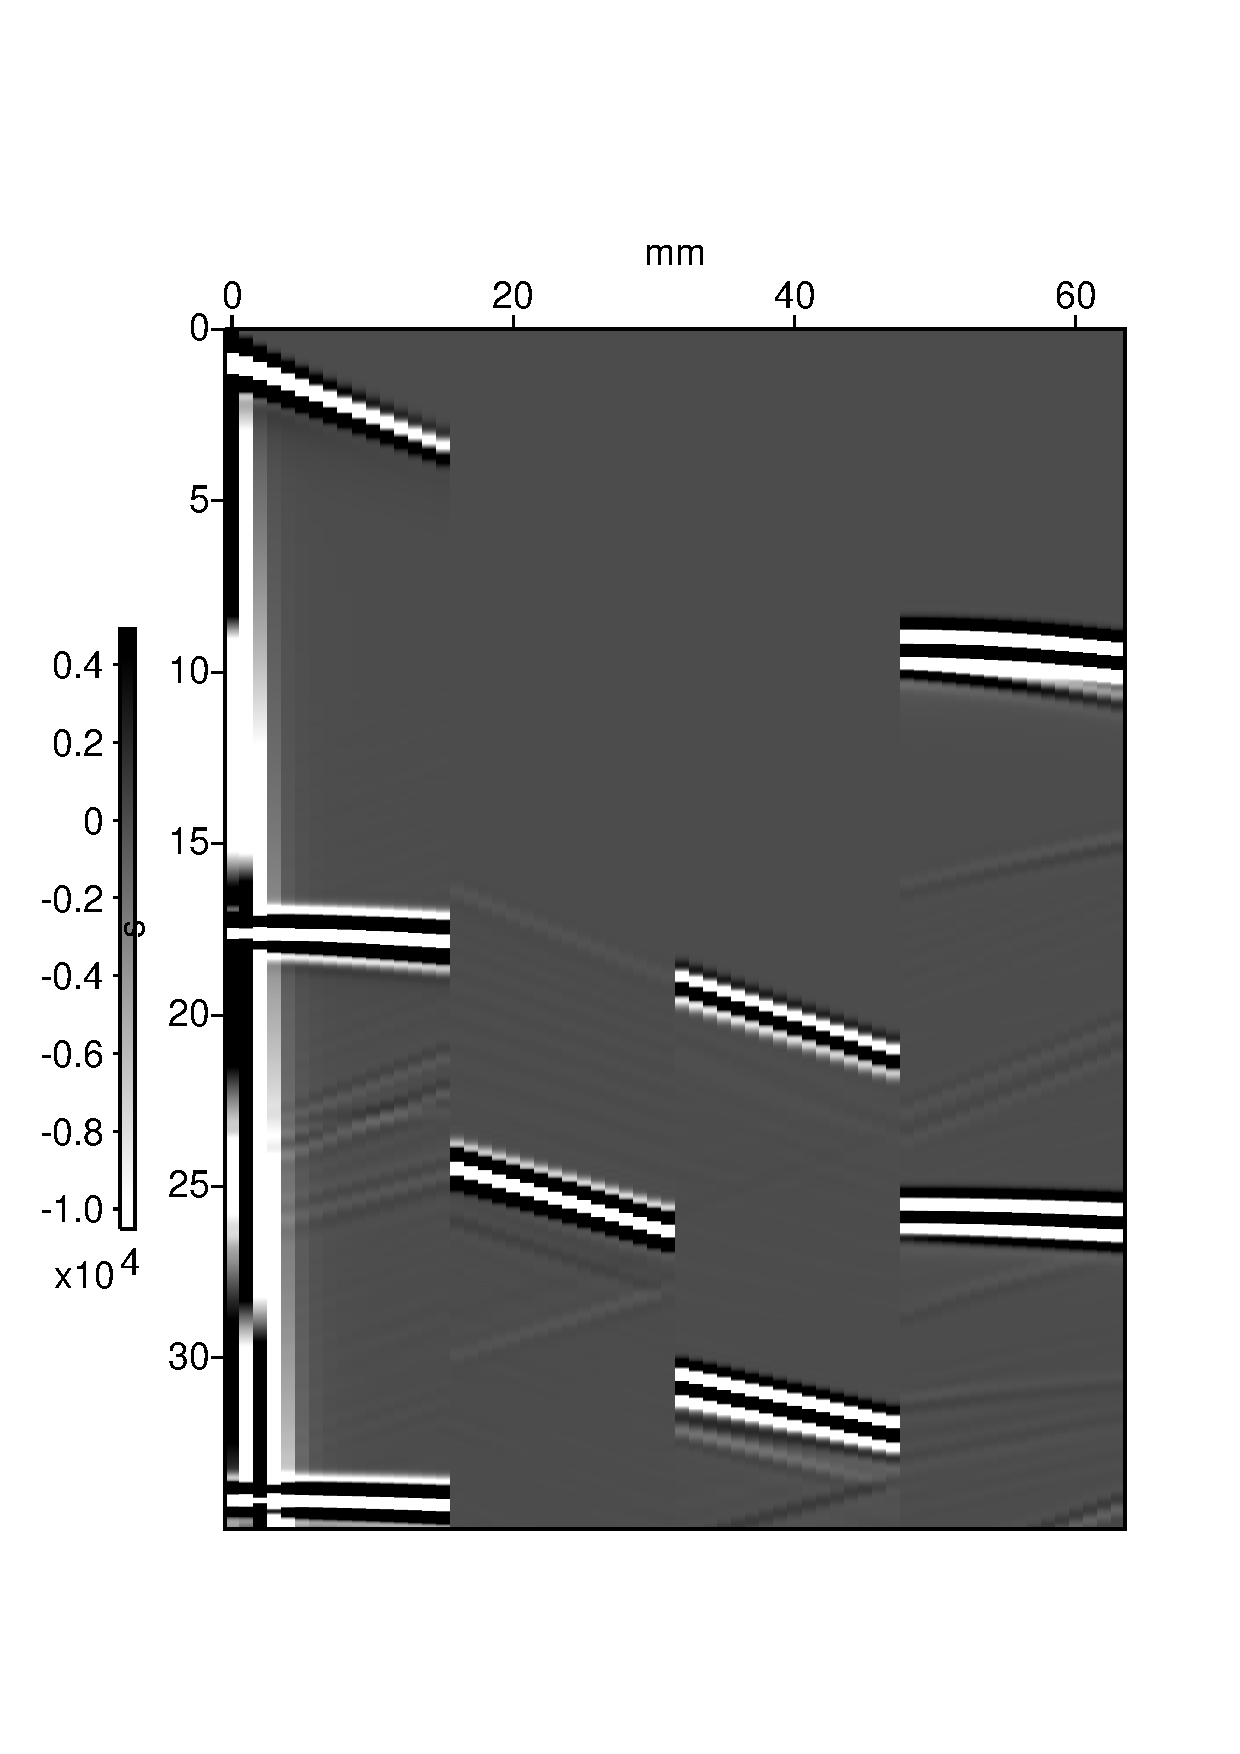
\includegraphics[width=\textwidth]{img/epsilon/e20.png}
		\caption{Données synthétiques.\label{app:ani:data_true}}
	\end{subfigure}
	\begin{subfigure}[b]{0.29\textwidth}
		\centering
		\includegraphics[width=0.91\textwidth]{img/epsilon/residu_init.png}
		\caption{Résidus initiaux. \label{app:ani:data_av}}
	\end{subfigure}
	\begin{subfigure}[b]{0.29\textwidth}
		\centering
		\includegraphics[width=0.91\textwidth]{img/epsilon/residu_final.png}
		\caption{Résidus finaux.\label{app:ani:data_ap}}
	\end{subfigure}
	\caption{ Signaux temporels et résidus acquis par les 4 barrettes, dont la numérotation correspond à celle de l'acquisition présentée en figure~\ref{app:ani:data_ap}. La source est le premier élément (le plus à gauche) de la barrette n° 1 et émet une excitation à 2 MHz.   L'échelle d'amplitude est la même pour les 3 figures. \label{app:ani:data}}
	\end{changemargin}


 Pour résumer, les données portent peu d'information sur l'anisotropie et ces informations permettent, au mieux, de reconstruire une image de très faible résolution. On sait qu'en pratique, le faisceau ultrasonore est très impacté par l'anisotropie. Il semble donc qu'un modèle de soudure anisotrope VTI soit donc trop restrictif pour représenter l'anisotropie d'une soudure réelle.\\
 
 Pour tester la capacité de la FWI à reconstruire ces paramètres d'anisotropie, il est donc nécessaire d'utiliser un modèle plus pertinent qui se rapprocherait davantage de celui développé par \cite{ogilvy} par exemple.	\cite{ogilvy} propose de simuler l'orientation des grains de la soudure avec un angle représenté sur la figure~\ref{ogilvy_soud}, tel que : 
	\begin{equation}
		\theta(x,z) = \tan^{-1}\left( \frac{D/2 + z\tan\alpha}{x} \right),
	\end{equation}
	avec $D$ la largeur de la racine de la soudure et $\alpha$  l'angle du bord de soudure. 
 
\begin{figure}[!h]
	\centering
			\includegraphics[width=4cm]{img/ogilvy_modele.png}
			\caption{ Exemple d'orientation de grains dans la soudure (image extraite de \cite{ogilvy}).\label{ogilvy_soud}}
\end{figure} 
 
%\begin{figure}[!h]
%	\begin{minipage}{0.34\textwidth}
%			\includegraphics[width=0.8\textwidth]{img/ogilvy_modele.png}
%			\caption{ Exemple d'orientation de grains dans la soudure (image extraite de \cite{ogilvy}).\label{ogilvy_soud}}
%	\end{minipage}
%	\hfill
%	\begin{minipage}{0.65\textwidth}
%	Pour tester la capacité de la FWI à reconstruire ces paramètres d'anisotropie, il est donc nécessaire d'utiliser un modèle plus pertinent qui se rapprocherait davantage de celui proposé par \cite{ogilvy} par exemple.\\
%	\cite{ogilvy} propose de simuler l'orientation des grains de la soudure avec un angle représenté sur la figure ci-contre, tel que : 
%	\begin{equation}
%		\theta(x,z) = \tan^{-1}\left( \frac{D/2 + z\tan\alpha}{x} \right),
%	\end{equation}
%	avec $D$ la largeur de la racine de la soudure et $\alpha$  l'angle du bord de soudure. 
%	\end{minipage}
%\end{figure}






\section{Enjeux et problématiques de l'inversion 3D élastique}

L'application de la FWI à des données réelles implique de prendre en compte la propagation en 3D des ondes dans la soudure. Une inversion 2D appliquée à de vraies données nécessite donc de les préconditionner de manière à limiter la trace des ondes de cisaillement et à leur appliquer une correction d'amplitude. \\

L'inversion 3D permet de prendre en compte l'ensemble des phénomènes de propagation et de tirer profit des ondes de cisaillement dont la longueur d'onde est plus faible que celle des ondes de compression. Cependant, les données peuvent être marquée par des ondes de surfaces dont l'atténuation est plus faible que les ondes de volume.  L'inversion est alors déséquilibrée par cette onde de forte amplitude et le modèle n'est mis à jour qu'en surface. L'influence de cette onde de surface sur les données peut être limitée par un filtrage adapté ou par une acquisition en transmission.\\ 

\todo[inline]{Mettre une image de comparaison des données 2D et 3D ? }
%élastique : 2 à 3 ordres de grandeurs plus cher en calcul. Pb moins bien posé : impose un modèle initial bien posé, ... Plus de paramètres impliqués=plus de degrés de liberté dans l'espace des modèles

L'acquisition peut être réalisée dans un plan, comme dans les cas présentés précédemment, ce qui risque de limiter la qualité de reconstruction hors de ce plan. Des structures 3D peuvent également être reconstruites par l'utilisation de transducteurs matriciels ou par déplacement d'un transducteur linéaire.




%%%%%%%%%%%%%%%%%%%%%notes%%%%%%%%%%%%%%%
%\todo[inline]{notes : \\
%
%anisotrope est plus problématique que isotrope car :\\ 
%-modélisation plus complexe,\\
%-problème moins bien posé\\
%
%Gholami 2011 : la vitesse a beaucoup plus d'influence sur les données que les paramètres delta et epsilon (delta étant le plus faible). D'après ses schémas, on va donc avoir une maj de la vitesse mais pas des autres paramètres\\
%
%modèle initial de soudure : citer mina ?\\

%VTI elliptique ne gène pas l'inversion car beaucoup d'info portées par la transmission (vecteurs d'ondes verticaux non affectés par l'anisotropie elliptique VTI)  -> pas assez proche du modèle réel

%le flop du vti montre que l'inversion des paramètres est tributaire de l'acquisition
%}




\addcontentsline{toc}{section}{\textbf{Conclusions}}
\chapter*{Conclusions}

L'état de l'art concernant l'imagerie de soudure montre que les images actuellement obtenues sont sujettes aux artefacts, ce qui peut poser des problèmes de sécurité pour les structures à risque. La FWI propose une approche non pas basée sur l'interprétation des temps de vol, mais sur l'utilisation de l'ensemble de l'enregistrement. Elle repose sur la résolution d'un problème inverse, ce qui lui permet de s'affranchir de la connaissance précise \emph{a priori} de la nature de l'anisotropie.\\

Ce travail a montré que la FWI peut donner des images d'une résolution de la moitié de la plus petite longueur d'onde propagée, dans le cas d'une propagation acoustique et d'une acquisition judicieusement choisie. L'anisotropie  décrite par un modèle acoustique transverse isotrope perturbe très peu la propagation des ondes, ce qui montre que cette anisotropie est trop éloignée de celle rencontrée dans les soudures réelles. Elle doit donc être décrite de manière plus complexe par une ensemble de constantes élastiques ou par un modèle transverse isotrope à axe de symétrie localement incliné.





La perspective de ce travail est l'application de la FWI à des données réelles, ce qui implique de prendre en compte la propagation en 3D des ondes dans la soudure. Une inversion 2D appliquée à de vraies données nécessite donc de les préconditionner de manière à limiter la trace des ondes de cisaillement et à leur appliquer une correction d'amplitude. \\

L'inversion 3D permet de prendre en compte l'ensemble des phénomènes de propagation et de tirer profit des ondes de cisaillement dont la longueur d'onde est plus faible que celle des ondes de compression. Cependant, les données peuvent être marquée par des ondes de surfaces dont l'atténuation est plus faible que les ondes de volume.  L'inversion est alors déséquilibrée par cette onde de forte amplitude et le modèle n'est mis à jour qu'en surface. L'influence de cette onde de surface sur les données peut être limitée par un filtrage adapté ou par une acquisition en transmission.\\ 


L'acquisition peut être réalisée dans un plan, comme dans les cas présentés précédemment, ce qui risque de limiter la qualité de reconstruction hors de ce plan. Des structures 3D peuvent également être reconstruites par l'utilisation de transducteurs matriciels ou par déplacement d'un transducteur linéaire.


L'inversion à partir de données réelles peut également nécessiter de considérer l'atténuation des ondes dans la soudure comme un nouveau paramètre du modèle, et d'estimer les sources au cours de l'inversion. La sensibilité au bruit de la FWI doit également être évaluée et la fonction de coût éventuellement adaptée \citep{brossier_2010}. La nature mal posée du problème d'optimisation peut nécessiter d'élaborer un modèle initial plus précis, construit statistiquement à partir d'un grand nombre de résultats d'inversion ou d'incorporer des \emph{prior informations} à la formulation de la fonction de coût \citep{asnaashari}.











%\subsection{améliorations}
%Le modèle initial choisi est très simple. Cependant, il serait intéressant d'utiliser statistiquement le résultats d'inversion de soudure pour construire un modèle initial plus complet ou incorporer des "prior informations" à la phase d'optimisation (\emph{i. e.} dans la formulation de la fonction de coût : cf \cite{asnaashari}).



%atténuation

%étude de sensibilité au bruit

%QUESTION : 
%Comment connaître l'incertitude, la réalité du résultat
%sensibilité au bruit
%Kirchhoff approx pour des défauts non pénétrables/gestion du contraste ? (materials and acoustics, p.421)

%\addcontentsline{toc}{section}{\textbf{Annexe}}
\chapter*{Annexe}

discrétisation
nombre d'itération
temps de calcul : pb direct qques secondes
inversion : 5 minutes pour 20 it à 1 freq avec 1 coeur par source


%\section{Note sur les dimensions des grandeurs du chapitre \ref{fwi}}
%
%Les matrice $A$, qui est l'opérateur de l'équation d'onde a les dimensions de l'espace du problème direct : $l\times l$, où $l=n_{x}\times n_{z}$, $n_{x}$ et $n_{z}$ étant les dimensions du milieu de propagation discrétisé.\\
% De la même façon, le champ d'onde $\bm{u}$ et le vecteur source $\bm{s}$ sont de dimension $l\times 1$.\\
%Or, les vecteurs de données $\bm{d}$ ne contiennent que les informations aux $n$ points de réception. Ils sont donc de dimension $1\times n$. Les calculs sont donc menés sur des vecteurs agrandis à l'aide de zéros de façon à ce que $\bm{d}$ soit de dimension $l\times 1$. \\
%Finalement, le gradient  $\frac{\dd C (\bm{m})}{\dd \bm{m}}$ est bien de dimension $M\times 1$ avec $M$ le nombre de paramètre du problème \citep{pratt_98}.



%%%%%%%% Biblio %%%%%%%%%%
\newpage

\bibliographystyle{plainnat}%\bibliographystyle{unsrt}
\bibliography{biblio}

\end{document} % fin doc


